\documentclass[11pt,a4paper]{report}
\usepackage[top=1in, bottom=1in, left=1in, right=1in]{geometry} % to change the page dimensions top=1in, bottom=1in, left=0.5in, right=0.5in,
\usepackage[utf8]{inputenc}
\usepackage[czech]{babel}
\usepackage[T1]{fontenc}
\usepackage{amsmath}
\usepackage{amsfonts}
\usepackage{amssymb}
\usepackage{graphicx}
\usepackage{epstopdf}
\usepackage{indentfirst}
%\setlength{\parindent}{4em} 
\author{Jakub Drápela}
\usepackage{fancyhdr}
\usepackage{siunitx}
\graphicspath{{./figures/}}

% pridano kvuli tabulkam 
\usepackage{array}
\newcolumntype{L}[1]{>{\raggedright\let\newline\\\arraybackslash\hspace{0pt}}m{#1}}
\newcolumntype{C}[1]{>{\centering\let\newline\\\arraybackslash\hspace{0pt}}m{#1}}
\newcolumntype{R}[1]{>{\raggedleft\let\newline\\\arraybackslash\hspace{0pt}}m{#1}}

\DeclareSIUnit\px{px}
\DeclareMathOperator*{\argmax}{arg\,max}

\makeatletter
\renewcommand{\@makechapterhead}[1]{%
\vspace*{20 pt}%
{\setlength{\parindent}{0pt} \raggedright \normalfont
\bfseries\Huge\thechapter.\ #1
\par\nobreak\vspace{20 pt}}}
\makeatother

%\fontfamily{phs}
%\selectfont
\usepackage[backend=bibtex,style=numeric,sortcites]{biblatex}
\usepackage{filecontents}  % create "citations.bib" on-the-fly
\begin{filecontents*}{thesis.bib}
@inproceedings{Matas,
   title = {Robust Wide Baseline Stereo from Maximally Stable Extremal Regions},
   author = {Matas, J. and Chum, O. and Urban, M. and Pajdla, T.},
   year = {2002},
   pages = {36.1-36.10},
   booktitle = {Proc. BMVC},
   isbn = {1-901725-19-7},
}
@ARTICLE{Comparison,
    author = {K. Mikolajczyk and T. Tuytelaars and C. Schmid and A. Zisserman and J. Matas and F. Schaffalitzky and T. Kadir and L. Van Gool},
    title = {A comparison of affine region detectors},
    journal = {International Journal of Computer Vision},
    year = {2005}
}
@thesis{Pohl2002,
  author       = {Petr Pohl},
  title        = {Simulace průletu paprsků transparentním objektem},
  type         = {phdthesis},
  institution  = {Czech Technical university in Prague},
  date         = 2002,
  location     = {Czech Republic},
  supervisor   = {Ing. Vladimír Smutný, Ph.D.},
}
@Book{bodlakLADOK,
  author =       {Bodlák, Igor},
  title =        {Rozšíření toolboxu LADOK, Semester project},
  publisher =    {Czech Technical University in Prague},
  year =         {2004},
}
@Book{strakaLADOK,
  author =       {Straka, Matěj},
  title =        {Tails of beam simulation in LADOK, Semester project},
  publisher =    {Czech Technical University in Prague},
  year =         {2013},
}
@thesis{Bodlak2005,
  author       = {Igor Bodlák},
  title        = {Modelování a analýza broušeného kamene},
  type         = {phdthesis},
  institution  = {Czech Technical university in Prague},
  date         = 2005,
  location     = {Czech Republic},
  supervisor   = {Ing. Vladimír Smutný, Ph.D.},
}
@thesis{Drapela,
  author       = {Jakub Drápela},
  title        = {Měření barevných broušených kamenů},
  type         = {phdthesis},
  institution  = {Czech Technical university in Prague},
  date         = 2015,
  location     = {Czech Republic},
  supervisor   = {Ing. Vladimír Smutný, Ph.D.},
}
@ARTICLE{SEXarticle,
   author = {{Bertin}, E. and {Arnouts}, S.},
    title = "{SExtractor: Software for source extraction.}",
 keywords = {METHODS: DATA ANALYSIS, TECHNIQUES: IMAGE PROCESSING, GALAXIES: PHOTOMETRY},
     year = 1996,
    month = jun,
   volume = 117,
    pages = {393-404},
   adsurl = {http://adsabs.harvard.edu/abs/1996A%26AS..117..393B},
  adsnote = {Provided by the SAO/NASA Astrophysics Data System}
}
@manual{SExtractorManual,
    author = {Bertin, E.},
    citeulike-article-id = {159020},
    citeulike-linkout-0 = {http://terapix.iap.fr/IMG/pdf/sextractor.pdf},
    keywords = {photometry, sextractor, software},
    organization = {Institud d'Astrophysique \& Observatorie de Paris},
    posted-at = {2017-03-14},
    priority = {0},
    title = {{SE}xtractor v2.5 User's Manual},
    url = {http://terapix.iap.fr/IMG/pdf/sextractor.pdf}
}
\end{filecontents*}
\bibliography{thesis}
%\addbibresource{thesis.bib}



\begin{document}
%\pagestyle{empty}
%
%%%nastaveni pisma  
%%\fontfamily{phv}
%%\selectfont
%
%	\begin{center}
%
%\large
%
%České vysoké učení technické v Praze
%
%\medskip
%
%Elektrotechnická fakulta
%\vfill
%\vfill
%{\LARGE\bfseries Detekce laserových stop v obraze}
%
%
%\vspace{15mm}
%
%\vfill
%\vfill
%\vfill
%
%\vfill
%
%\begin{tabular}{rl}
%
%Autor: & Jakub Drápela \\
%\noalign{\vspace{2mm}}
%Studijní obor: & Kybernetika a robotika \\
%\noalign{\vspace{2mm}}
%Datum vypracování: & \today\\
%\end{tabular}
%
%\end{center}
%
%\newpage
\pagestyle{plain}     % zapne obyčejné číslování
\setcounter{page}{1}  % nastaví čítač stránek znovu od jedné  
\chapter{Úvod}

Drahé kameny jsou lidstvem od pradávna vyhledávány.
Jsou znakem krásy, bohatství a moci. Z počátku se kameny leštily do oblých tvarů a stávaly se součástí šperků.
S vývojem civilizace se začaly drahé kameny brousit, aby se zvýraznil lom světla a lesk minerálu. Broušením vznikaly rovinné fasety. Kombinací faset s definovanou velikostí a sklonem se vyvinuly standardní tvary jako brilliant, trilliant, rosette,baguette apod. Drahé a velmi cenné suroviny jako diamant se brousí pouze ručně. Méně významné kameny jsou převážně opracovávány automatickými stroji.  

Cenu broušených kamenů určují čtyři základní parametry. Mezi ně patří čistota, barva, hmotnost a kvalita brusu. 

Čistota určuje množství příměsí v materiálu kamene. Při tvorbě krystalu mohou dále vzniknout praskliny či vzduchové bubliny. 

Broušené kameny dělíme do široké řady odstínů. Barva kamene závisí jeho chemickém složení. Důležitá je v tomto ohledu jednotnost barev.

Hmotnost souvisí s velikostí kamene. U diamantů se hmotnost určuje v karátech  a je natolik důležitá, že se v některých případech volí kompromis mezi kvalitou brusu.

Brus je důležitá mechanická úprava kamene. Ideálně opracovaný kámen má dokonalý soulad mezi brilancí, ohněm a jiskřením. Mezi parametry hodnotící kvalitu brusu patří kvalita povrchového opracování faset. Fasety se brousí rovinnými brusnými kotouči. Broušením mohou vzniknout rýhy, škrábance, prohlubně, abraze na hranách (zbroušení přechodu mezi fasetami), povrchová oxidace a nové fasety. Kámen je třeba brousit s vysokou přesností. Každá odchylka velikosti a úhlu fasety od ideálního tvaru zhorší optické vlastnosti kamene. Orientace faset je proto důležitým parametrem pro zhodnocení kvality brusu.

Jedním z nástrojů ke zkoumání optických vlastností broušeného kamene je nasvícení jeho povrchu světelným svazkem. Na fasetách broušeného kamene dochází ve zjednodušeném případě k odrazu a lomu světelného svazku. Z toho důvodu se dopadající svazek roztříští na řadu světelných svazků různých tvarů. Svazky jsou definovány směrem šíření, zářivým tokem a elektromagnetickými parametry. 

Barva, čistota a kvalita brusu mají za následek změnu geometrie svazků. Ta je jednoznačným popisem broušeného kamene. Hodnocením vystupujících svazků můžeme určit parametry kamene. 

Tato práce navazuje na dlouhodobý výzkum v Centru strojového vnímání na katedře kybernetiky Elektrotechnické fakulty ČVUT. 


První práce, která se zabývá průchodem nerozbíhajícího se svazku konvexním tělesem je software LADOK \cite{Pohl2002} od Petra Pohla.  

Práce využívá software LADOK \cite{Pohl2002} od Petra Pohla. Simulační program LADOK zavádí pro broušený kámen geometrický model ve formě konvexního mnohostěnu s rovnými ploškami, fasetami. Na povrch kamene dopadá svazek nerozbíhajících se paprsků světla z definovaného směru. LADOK řeší odrazy, lomy a dělení svazků na povrchu kamene. Svazky po opuštění kamene mají definovaný směr, zářivý tok, plochu a tvar. Tento software rozšířil Igor Bodlák \cite{bodlakLADOK} o výpočet elekromagnetické vlastnosti svazků. Matematický model kamene obohatil Martin Straka \cite{strakaLADOK}. Přechody mezi fasetami modeloval jako posloupnost většího počtu menších faset s nenulovým poloměrem křivosti. 

LADOK je matematickým řešením experimentu na obr. \ref{fig:basicMeasure}. Zdrojem světla je laser. Laserový svazek dopadá na broušený kámen, kde se roztříští na mnoho menších svazků. Ty jsou po opuštění kamene zachyceny na stínítku. Stínítko snímáme kamerou a získáváme obraz svazků na stínítku.  


\begin{figure}[h!]
\begin{center}
\scalebox{0.5}{ \input{xfig/stinitko.pstex_t}}
\end{center}
\caption{Nákres principu experimentu. Laser produkuje svazek světla, který dopadá na celou plochu kamene. V kameni se svazek roztříští na mnoho svazků. Svazky vystupující z kamene v horní polorovině dopadnou na stínítko. Stínítko snímá kamera. Převzato z \cite{Drapela}.}
\label{fig:basicMeasure}
\end{figure}


Experimentální soustavu máme sestavenou a zkalibrovanou \cite{Drapela}. Známe transformaci mezi obrazem svazku na stínítku a směrem, ve kterém opouští kámen. 

O možnost porovnání dat reálného experimentu s výsledky počítačové simulace se postaral Igor Bodlák \cite{Bodlak2005}. Navrhl optimalizaci kritéria hodnotící rozdíl vzdálenosti stop z experimentu a odrazů stop simulace na stínítku. Optimalizovaly se parametry faset kamene a kámen se tak deformoval, aby se dosáhlo co nejlepší shody v zadaném kritériu. Software pro řešení inverzní úlohy nazval zkratkou LAM. 

LAM byl použitelný pouze pro broušený kámen čtvercového tvaru. Z důvodu složitosti přiřazení stop z experimentu k obrazům simulovaných svazků při osvětlení celého kamene zaměřil vstupní laserový svazek pouze do určitých míst kamene. Tím vzniklo redukované množství svazků a korespondence se simulovanými svazky se výrazně zjednodušila. Nevýhodou tohoto přístupu jsou rozměry kamene, které musí být několikanásobně větší než průměr laserového svazku. Metoda je prakticky nepoužitelná pro kameny o rozměrech v jednotkách milimetru. 

	V této práci osvítíme laserovým svazkem celý kámen. Zaměříme se na kameny šatonové růže s plochým spodkem a 12-ti bočními fasetami. Tyto kameny se ve zkratce nazývají \textit{viva12}. Rozměry kamenů budou v řádech milimetrů. 
	
	K robustní detekci obrazu svazků použijeme MSER detektor \cite{Matas}. Z výsledku detekce určíme parametry stop. Sestavíme program, pomocí kterého bude možno manuálně párovat obrazy svazků broušeného kamene se simulovanými stopami.
 Optimalizací z LAMu získáme náklony faset. Parametry svazků prozkoumáme pomocí určených experimentů. Navrhneme algoritmus pro \textit{vivu12}, který určí automaticky orientaci faset kamene. Výstupem programu budou odchylky úhlů faset kamene od jejich ideální pozice.


















\chapter{Fyzikální model}

\section{Model kamene}
Broušený kámen je modelován jako konvexní mnohostěn \cite{Pohl2002}. Brusné kotouče považujeme za dokonale rovinné. Uchycení kamene při broušení zjednodušíme na absolutně tuhé bez známek pružnosti či ohybu. Fasety potom můžeme modelovat jako rovné plochy. Orientace a umístění fasety získáme z výkresu nebo předchozího měření. 

Přechody mezi fasetami jsou v ideálním případě ostré hrany. Z důvodu abraze hran v procesu výroby kamene jsou hrany obroušeny do oblého tvaru. K přiblížení modelu reálnému obroušení hran aproximujeme hranu množstvím rovinných faset se vzájemnou polohou odpovídající poloměru křivosti hrany.  
  
\begin{figure}[htps]
\centering
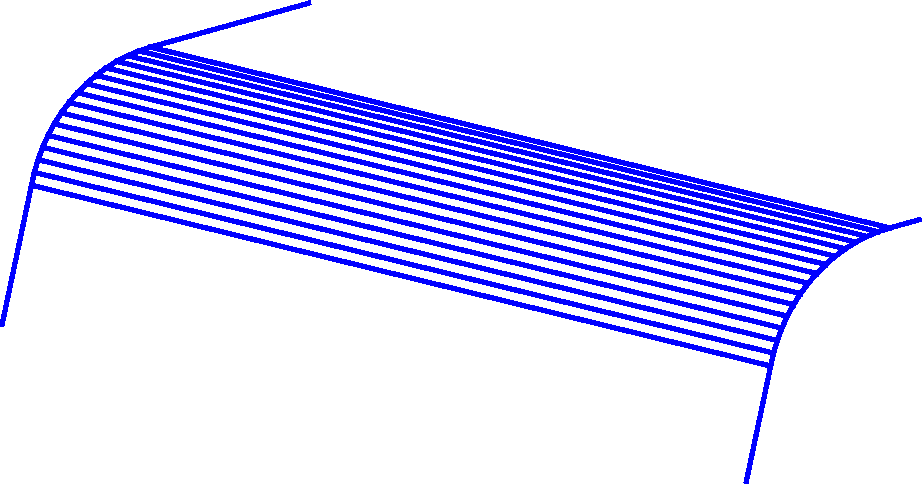
\includegraphics[width=0.6\linewidth]{edge_ex.pdf}
\caption{Detail aproximace přechodu mezi fasetami.}
\label{fig: edge}
\end{figure}  

\section{Model svazku}
Svazek světla v LADOKU reprezentuje nerozbíhající se konvexní hranol. Vlivem odrazu a lomu se konvexní tvar zachová. Fasety jsou také konvexní, proto se konvexita zachová i při štěpení svazku. Po opuštění kamene jsou svazky definovány zářivým tokem, plochou a směrem, které lze vyjádřit pomocí azimutu a elevace. Stokesovy koeficienty definují elektromagnetické vlastnosti svazku. 

Zaznamenána je celá cesta svazku. V každém bodě trasy máme k dispozici posloupnost směrů a tvarů svazku vyjádřeném pomocí polygonu. 

Model nepostihuje situace, při kterých nastává rozbíhavost světla.
\begin{itemize}
\item Pokud jsou v materiálu přítomné nečistoty, praskliny, vzduchové bubliny apod., světelný svazek se rozptýlí.
\item  Rozptyl světelných svazků vzniká vlivem nedokonalého vyleštění faset a to jak při lomu tak při odrazu.
\item Vlivem oxidace při leštění mohou vzniknout místa s jiným indexem lomu než je index lomu materiálu. Podobný případ nastane pokud má kámen nejednotný odstín.

\item Přítomnost hran v kameni způsobí ohyb světla (difrakci).
\end{itemize}

Část zářivého toku svazku může být pohlcena a přeměněna na teplo.

\section{Model stínítka}
\label{sec:stinitko}
Po dopadu laserového svazku na stínítko se záření difuzně odrazí. Odrazivé vlastnosti materiálu závisí na úhlu odpadajícího světla a lze je matematicky popsat pomocí modelu zvaného BRDF (Bidirectional reflectance distribution function). Odražené světlo zvýší intenzitu světla nejen v místě dopadu světelného svazku, ale i v jeho okolí.

Odražené světlo zároveň putuje do kamene a od něj zpět na stínítko. 

%%tohle bych zařadil na později
%Laserové stopy chceme detekovat v černobílém HDR snímku půlkulového stínítka, na které dopadá část laserových svazků vystupujících z nasvíceného kamene. Snímek ze zatížen radiálním zkreslením, které je způsobeno vlastností optické soustavy objektivu. Radiální zkreslení bylo určeno v předchozí bakalářské práci \cite{Drapela}. Snímek lze pomocí transformace z \cite{Drapela} zkreslení zbavit. Z \cite{Drapela} navíc známe transformaci mezi pozicí bodu v nezkresleného snímku a odpovídajícím parametrům azimutu a elevace.



V ideálním případě lze ve snímaném obraze pozorovat pouze dopady světelných svazků, které vznikly kombinací odrazů a lomů zdrojového svazku od faset broušeného kamene. U reálného kamene ovšem v obraze pozorujeme tenké slábnoucí přímky vycházející ze stopy světelného svazku, ocásky. Tyto ocásky vznikají díky lomu/odrazu světelného svazku od neostrých hran broušeného kamene.

\begin{figure}[h!]
\begin{center}
\scalebox{.9}{ \input{xfig/tails.pstex_t}}
\end{center}
\caption{Příklad snímaného obrazu s vyznačením obrazů svazků a ocásků.}
\label{fig:tail_ex1}
\end{figure}


Vnik ocásků si ukážeme při lomu světla na oblé hraně kamene. Situaci budeme uvažovat v 2D prostoru, kde platí obecně stejné principy jako ve 3D. Světlo nahradíme paprsky světla se směrem šíření $\vec{v_i}$. 

Zvolíme si dvě fasety, které svírají úhel \SI{45}{\celsius}. Ostrý přechod aproximujeme. Vznikne posloupnost úseček, které propojují fasety. Každé úsečce přiřadíme normálový vektor $\vec{n}$.  

\begin{figure}[htp]
\centering
\begin{minipage}[c]{0.48\textwidth}
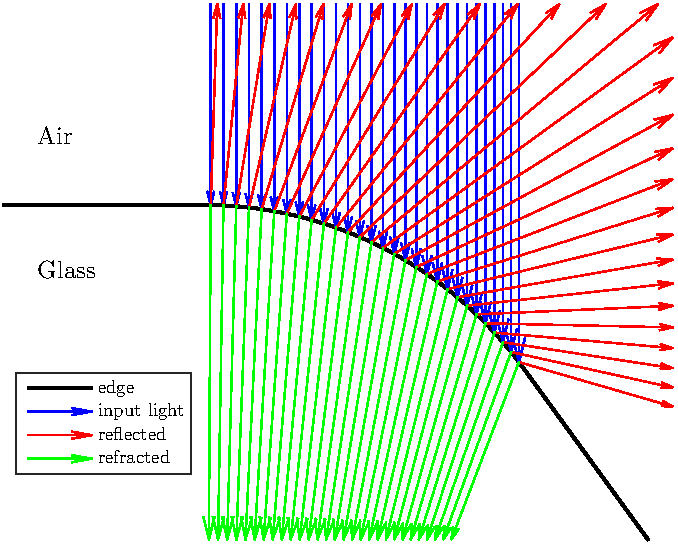
\includegraphics[width=\textwidth]{edgeIn.pdf}
\end{minipage}
\begin{minipage}[c]{0.48\textwidth}
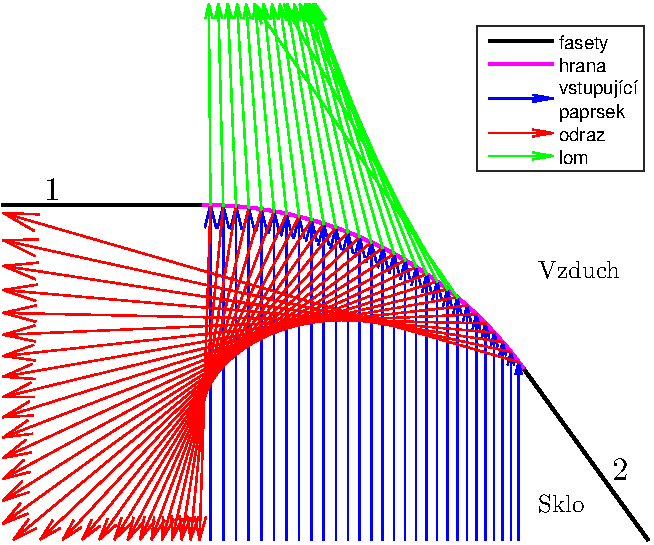
\includegraphics[width=\textwidth]{edgeOut.pdf}
\end{minipage}
\caption{Dopad světelných paprsků na hranu. Paprsky se lomí vlevo ze vzduchu do skla a vpravo ze skla do vzduchu. Situace pro index lomu vzduchu $n_a = 1$ a index lomu skla $n_g = 1.5$.}
\label{fig:edgeIn}
\end{figure}
Z Fresnelových rovnic víme, že dochází nejen k lomu světla, ale část světla000 se odrazí. Poměr intenzity odraženého a lomeného světla závisí na polarizaci světla a dopadajícím úhlu. V této ukázce uvažujeme nepolarizované světlo. 

Aplikací Snellova zákonu a zákonu odrazu na $\vec{n}$ a $\vec{v_i}$ vypočítáme směr lomu a odrazu světelných paprsků.

Na obr. \ref{fig:edgeIn} dopadají paprsky světla ze vzduchu na sklo i ze skla do vzduchu. V odou případech se odražené i lomené paprsky projeví jako ocásky.

Pokusíme se prozkoumat intenzitu ocásků $I$ v závislosti na vystupujícím úhlu, elevaci $\varepsilon$. 
Pro jednotlivou elevaci určíme intenzitu relevantně ke vstupující intenzitě jako 
\begin{equation}
 I_\varepsilon  = \frac{\rho_{{max}}}{\rho_\varepsilon}\cdot R
\end{equation}
pro odražené paprsky a 
\begin{equation}
 I_\varepsilon  = \frac{\rho_{\varepsilon_{max}}}{\rho_\varepsilon}\cdot (1-R)
\end{equation}
pro lomené paprsky, kde  

	\begin{tabular}{l l}
	$\rho_{\varepsilon}$ & 	- hustota paprsků pro danou elevaci $\varepsilon\,$,\\
	$\rho_{{max}}$  	&	- maximální hustota paprsků ve všech elevacích,\\
	$R_\varepsilon$		&	- odrazivost z Fresnelových rovnic pro $\varepsilon\,$.	 \\
	
	\end{tabular}

Závislost $I(\varepsilon)$ je označená jako \textit{Reflection coefficient} resp. \textit{Refraction coefficient} na obrázcích \ref{fig:edgeInGraf} a \ref{fig:edgeOutGraf}.


\begin{figure}[htps]
\centering
\begin{minipage}[c]{0.48\textwidth}
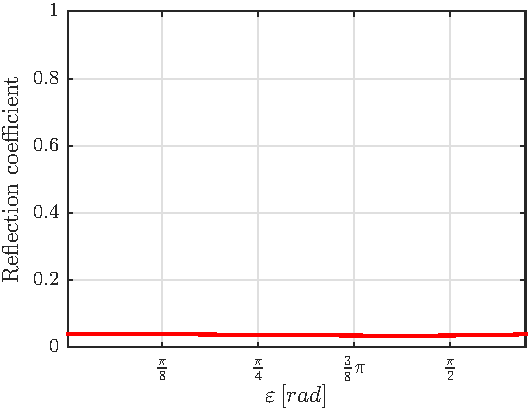
\includegraphics[width=\textwidth]{edgeIn_reflection.pdf}
\end{minipage}
\begin{minipage}[c]{0.48\textwidth}
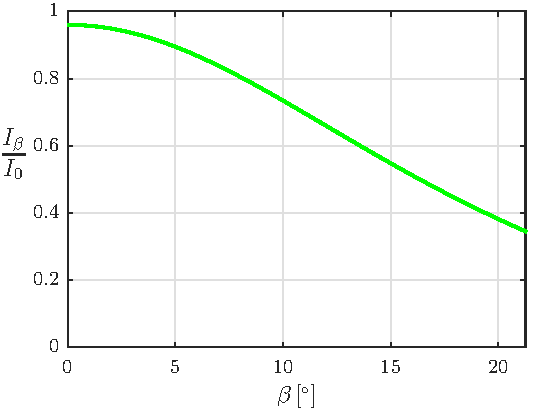
\includegraphics[width=\textwidth]{edgeIn_refraction.pdf}
\end{minipage}
\caption{\textit{Reflection coefficient} resp. \textit{Refraction coefficient} v případě když se lomí světlo ze vzduchu do skla (obr. \ref{fig:edgeIn}).}
\label{fig:edgeInGraf}
\end{figure}

\begin{figure}[htps]
\centering
\begin{minipage}[c]{0.48\textwidth}
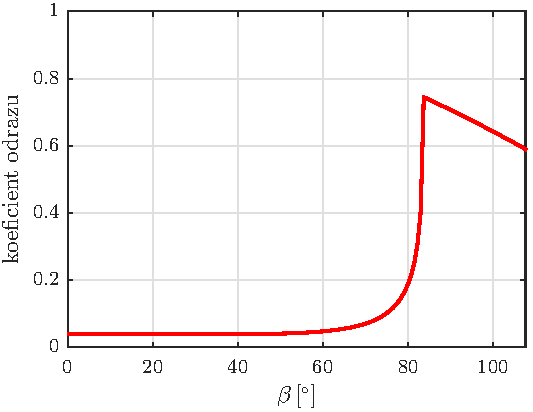
\includegraphics[width=\textwidth]{edgeOut_reflection.pdf}
\end{minipage}
\begin{minipage}[c]{0.48\textwidth}
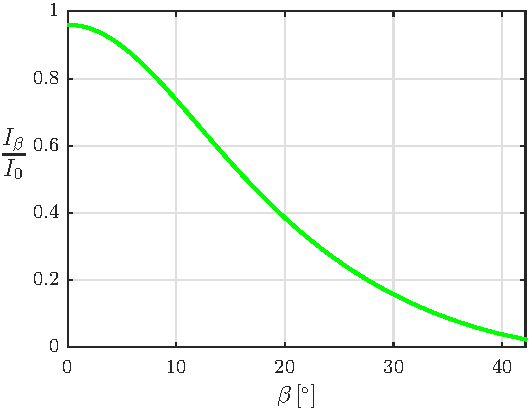
\includegraphics[width=\textwidth]{edgeOut_refraction.pdf}
\end{minipage}
\caption{\textit{Reflection coefficient} resp. \textit{Refraction coefficient} v případě když se lomí světlo ze skla do vzduchu (obr. \ref{fig:edgeIn}).}
\label{fig:edgeOutGraf}
\end{figure}

Z grafů \ref{fig:edgeInGraf} a \ref{fig:edgeOutGraf} je patrné, že ocásky budeme pozorovat různě dlouhé a z vysokou variabilitou z hlediska intenzity. 
	  

 Intenzita a délka ocásku je ovlivněna i dalšími faktory, jako je např. délka hrany, čistota hrany, drsnost povrchu atd. Všechny faktory, které ovlivňují intenzitu ocásku prozatím nejsme schopni v programu LADOK zahrnout do matematického modelu, proto pro prování svazků bude užitečná především informace o směru ocásku. 
 
 

\section{Model obrazu}

Obraz snímaný kamerou je zatížen radiálním zkreslením. Zkreslení odstraníme pomocí kalibrace kamery \cite{Drapela}. 


\section{Model Kamery}
\label{sec:poisson}
 Použitý CCD snímač má $2050^2$ pixelů. Každému pixelu odpovídá jeden samostatný snímač, který funguje na principu počítání přicházejících fotonů po dobu expozice. Počet přicházejících fotonů v daném časovém intervalu se řídí Poissonovým rozdělením. Pravděpodobnost, že napočítáme $n$ fotonů je 
 
 \begin{equation}
    P(\mathrm{X} = n)=\frac{\lambda ^{n}\,\mathrm{e}^{-\lambda}}{n!}\,,
 \end{equation}
 kde $\lambda$ je střední hodnota a $\mathrm{X}$ náhodná veličina.













\part{Detekce světelných stop v obraze}
\label{sec:detection}

\section{Jevy v obraze}
Pro analýzu vlastností broušeného kamene je důležité detekovat světelné stopy vzniklé dopadem laserových svazků na stínítko. Zároveň je třeba určit parametry stop, které se budou porovnávat s parametry svazků matematického modelu kamene. 

Intenzitu pixelu $I$ můžeme vyjádřit pomocí Poissonova rozdělení jako 
\begin{equation}
	I = \mathrm{Pois}\left(I_{s}+I_{p}+I_{o}\right)\,,
	\label{eq:intensitu_sum}
\end{equation}
 kde $I_{s}$ reprezentuje příspěvek světelného svazku, $I_{p}$ intenzitu pozadí, $I_{o}$ intenzitu světelných ocásků. Jedním z úkolů detektoru je oddělit pozadí od zbývajících složek intenzit. %Po odečtení pozadí získáme obrazy laserových svazků.   
 
Jednoduchým postupem pro určení intenzity pozadí by bylo prahování obrazu nad konstantní úrovní. V našem obraze však typicky konstantní není (kapitola \ref{sec:stinitko}). 

\begin{figure}[h!]
\centering
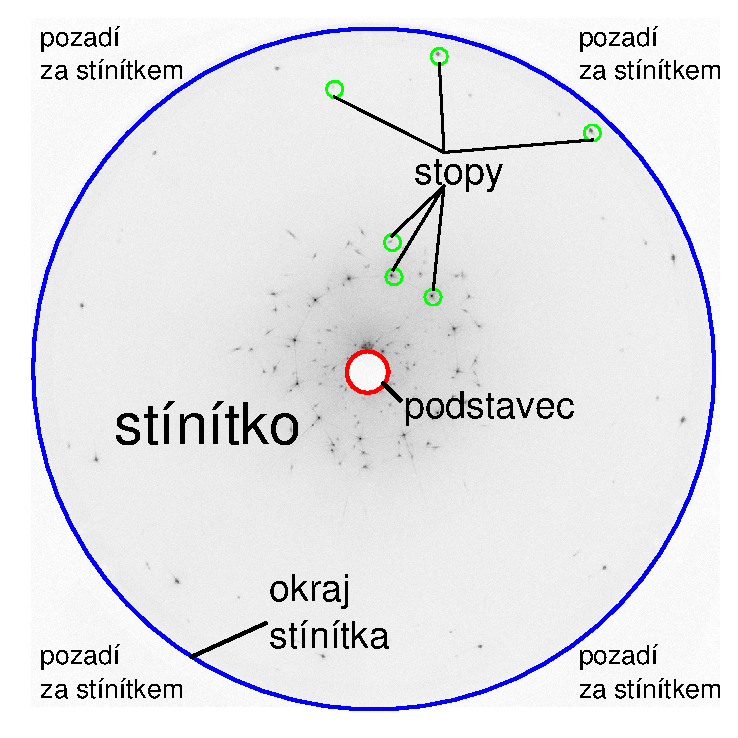
\includegraphics[width = 0.5\textwidth]{stinitkoSnimek.eps}
\caption[Popis objektů v obraze.]{Popis objektů v obraze.}
\label{fig: podstavec}
\end{figure}


Rozdílné pozadí se může také vytvořit odrazem zdrojového svazku od jiných předmětů, než broušeného kamene. Hlavním příspěvkem je v tomto případě odraz od podstavce, na který pokládáme broušený kámen (obr. \ref{fig: podstavec}).

\begin{figure}[h!]
\centering
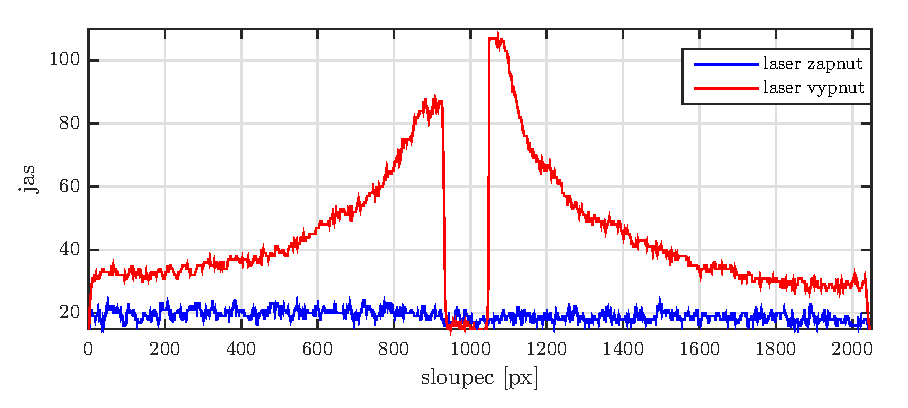
\includegraphics[width = 0.6\textwidth]{podstavec.eps}
\caption[Vliv odrazu od podstavce na pozadí snímku.]{Jasové úrovně ve vybraném řádku obrazu. Řádek protíná obraz podstavce. V případě červené charakteristiky dopadá na podstavec laserový svazek, rozptyluje se a dopadá na stínítko. Modrou charakteristiku pozorujeme, pokud je laser vypnutý.}
\label{fig: podstavec}
\end{figure}

Hodnotu pozadí potřebujeme znát, abychom ze snímku mohli vypočítat světelný tok pro jednotlivé dopadající laserové svazky. Určení intensity pozadí v každém pixelu komplikuje obraz podstavce na kámen a okolí stínítka. Zde je intenzita světla podstatně nižší, než na povrchu stínítka. Vysoká změna jasu v obraze komplikuje určení pozadí.  

V okolí stínítka můžeme detekovat falešné svazky, které je třeba odstranit. 

Světelné stopy se mohou překrývat. Pro odlišení příspěvků jednotlivých svazků je třeba obraz prahovat v několika úrovních jasu.

V místě, kde je vysoká koncentrace svazků mohou svazky dopadnout tak blízko sebe, že splynou v jednu stopu (obr. \ref{Splynuti}).  

\begin{figure}[h!]
    \centering
    \begin{minipage}[c]{0.48\textwidth}
        \centering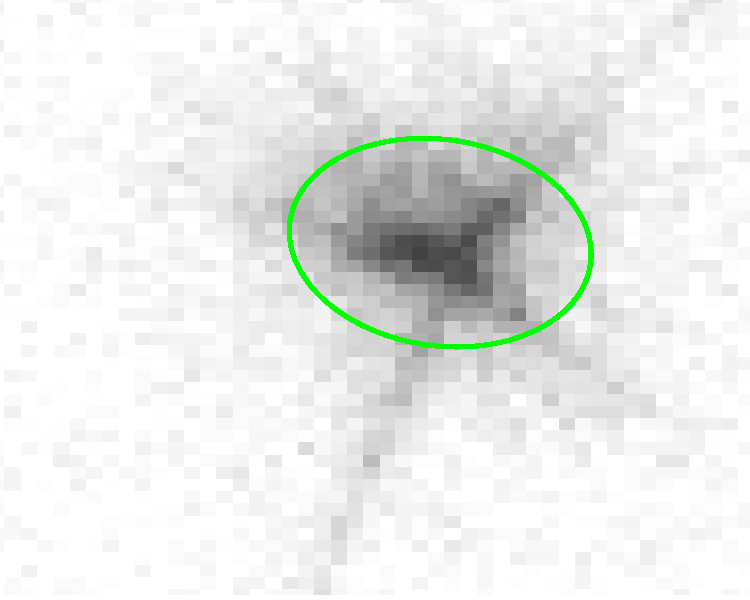
\includegraphics[width=.5\textwidth]{pf_near.pdf}
    \end{minipage}
    \begin{minipage}[c]{0.48\textwidth}
        \centering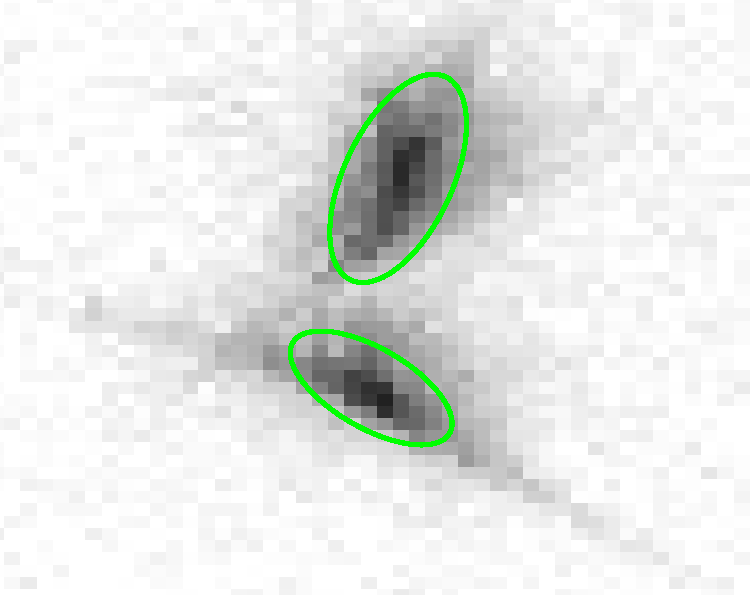
\includegraphics[width=.5\textwidth]{pf_near2.pdf}
    \end{minipage}
    \\
        \caption[Slynutí dvou různých svazků.]{Ilustrace slynutí dvou různých svazků. V pravém i levém snímku se nachází typově stejné laserové svazky. Na levém obrázku dopadly na stínítko příliš blízko sebe. V tomto případě nejsme schopni rozlišit příspěvek obou svazků a detekujeme pouze jednu stopu.}
        \label{Splynuti}
\end{figure}

Obraz je třeba filtrovat. Filtrováním snížíme šum v odraze, ale zároveň zmenšíme kontrast mezi stopami. 

Ne všechny svazky vystupující z kamene je možné detekovat. Svazky s vícenásobným odrazem postupně ztrácí zářivý tok. Po dopadu na stínítko mohou být nerozlišitelné od šumu a jejich detekce je prakticky nemožná. Pro stopy s nízkým jasem bude detekce často selhávat.

\begin{figure}[h!]
    \centering
    \begin{minipage}[c]{0.48\textwidth}
        \centering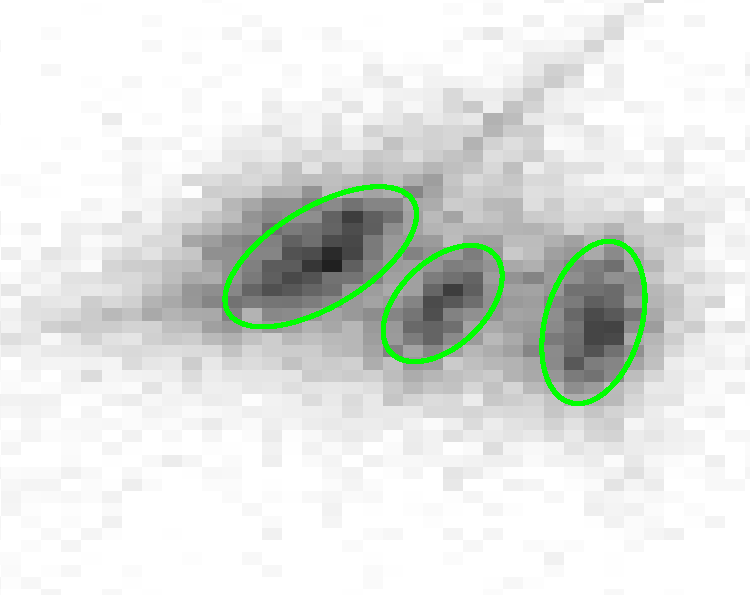
\includegraphics[width=.75\textwidth,height = 4.5 cm]{pf_punch2.pdf}
    \end{minipage}
    \begin{minipage}[c]{0.48\textwidth}
        \centering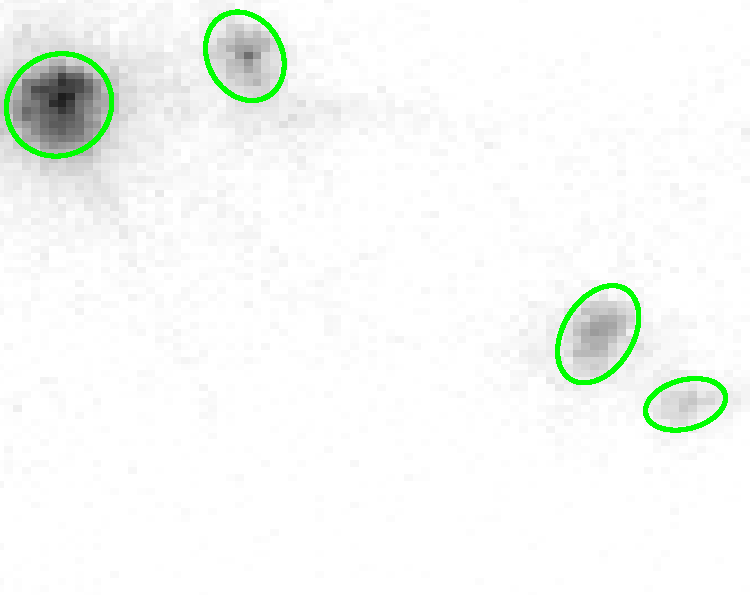
\includegraphics[width=.75\textwidth,height = 4.5 cm]{p_deff2.pdf}
    \end{minipage}
    \\
        \caption[Problémové detekce.]{Problémové detekce. Nalevo jsou laserové stopy blízko u sebe. Stopy je nutné od sebe oddělit. Na levém snímku jsou znázorněny výrazné rozdíly mezi velikostí a intenzitou stop. Je nutné použít víceúrovňový detektor. }
        \label{fig:Detekce}
\end{figure}

\newcommand\x{4}
\newcommand\xx{0,155}

\begin{figure}[h!]
    \centering
    \begin{minipage}[c]{0.163\textwidth}
        \centering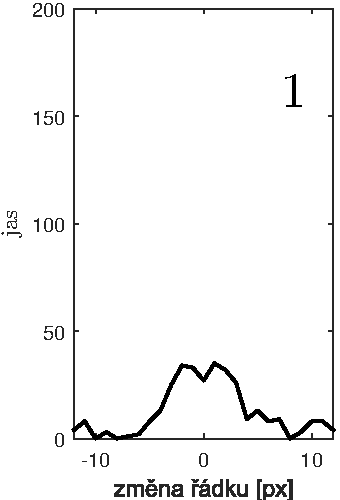
\includegraphics[height = \x cm,width = \textwidth ]{cut_1.pdf}
    \end{minipage}
    \begin{minipage}[c]{\xx \textwidth}
        \centering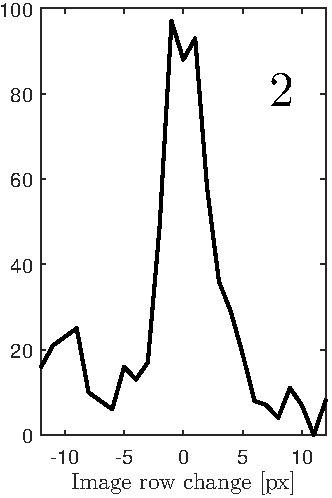
\includegraphics[height = \x cm,width = \textwidth]{cut_2.pdf}
    \end{minipage}
    \begin{minipage}[c]{\xx \textwidth}
        \centering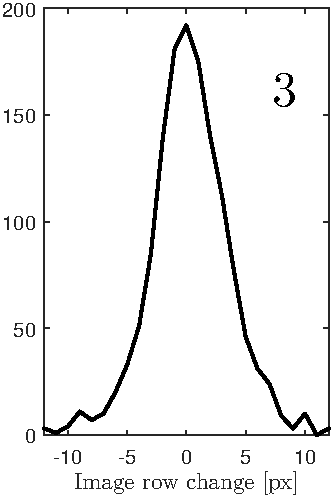
\includegraphics[height = \x cm,width = \textwidth]{cut_3.pdf}
    \end{minipage}
    \begin{minipage}[c]{\xx \textwidth}
        \centering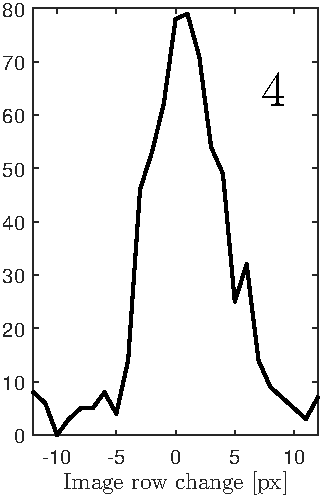
\includegraphics[height = \x cm,width = \textwidth]{cut_4.pdf}
    \end{minipage}
    \begin{minipage}[c]{\xx \textwidth}
        \centering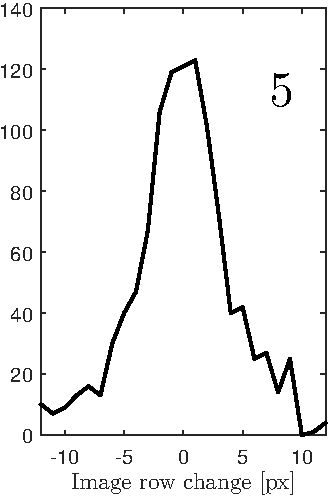
\includegraphics[height = \x cm,width = \textwidth]{cut_5.pdf}
    \end{minipage}
    \begin{minipage}[c]{\xx \textwidth}
        \centering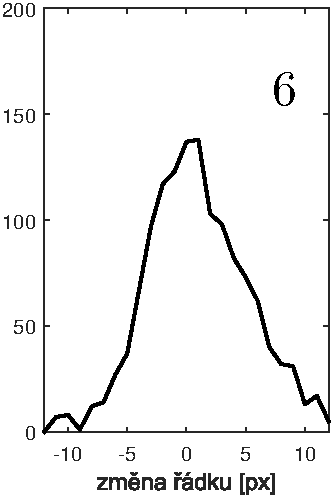
\includegraphics[height = \x cm,width = \textwidth]{cut_6.pdf}
    \end{minipage}
    \\
        \caption[Jasové řezy.]{Jasové řezy ve totožném sloupci obrazu. Řez protíná pixel s maximální hodnotou jasu ve stopě. Číslování řezů odpovídá indexům stop na obr. \ref{fig:Detekce}.}
        \label{fig:rezy}
\end{figure}


\section{Předchozí práce}

V předchozí práci \cite{Drapela} jsme neměli možnost detekovat stopy s nízkým jasem. Překrývající se svazky bylo nemožné oddělit.  

Bohatší pojetí problému se objevilo v Bodlákově práci \cite{Bodlak2005}. Snímek se prahoval více než jedním prahem. Z oblastí nad prahem se sestavila stromová struktura. Světelné stopy se určily jako listy stromu s dostatečnou významností. Tento přístup je však pro svou výpočetní náročnost nepoužitelný pro snímky s rozlišením 2050$\times$2050, které máme k dispozici. 

Naše úloha detekce je velmi podobná detekci hvězd a galaxií v astronomických snímcích. V oblasti astronomie se hojně používá program s názvem Source Extractor \cite{SEXarticle}. Tento program má za sebou dlouholetý vývoj, je optimalizován z hlediska rychlosti a odzkoušený širokou veřejností. Tento software lze po naladění parametrů použít i pro náš případ. Nevýhodou však je, že nelze spustit v operačním systému Windows, který využíváme.  

Po testu různých detektorů jsme se rozhodli pro detekci laserových stop v obraze využít relativně nový přístup uveden J. Matasem et al. \cite{Matas} v roce 2002 - MSER detektor. 




\section{MSER (maximal stable extremal region) detektor}

MSER detektor hledá v obraze maximálně stabilní extrémní oblasti. Původně byl využit pro robustní nalezení korespondencí mezi dvěma snímky stejného objetu pořízených z různého místa a v současné době se používá v mnoha oblastech počítačového vidění.  

Princip spočívá v několikaúrovňovému prahování obrazu podle intenzity a nalezení spojitých oblastí, které jsou nad či pod prahovou hodnotou. Mezi úrovněmi jsou nalezeny korespondující oblasti a za MSER oblasti jsou označeny ty, jejichž velikost z předchozí úrovně se se zvyšující úrovní příliš nezměnila. 

Výhodou MSER detektoru je invariance vůči afinní transformaci intenzity a vůči změně měřítka, což umožňuje současnou detekci malých a velkých oblastí s různou intenzitou. Podle studie \cite{Comparison}, která porovnává MSER detektor s ostatními typy detektorů významných oblastí, dosáhl MSER detektor skvělých výsledků v detekci oblastí s vysokou hustotu a variabilní změnou velikosti. MSER detektor se tedy zdá být vhodným kandidátem pro detekci laserových stop v obraze.

\section{Implementace}

\subsection{Filtrace}
   Nejprve se pokusíme minimalizovat Poissonův šum v obraze. Šum redukujeme konvolucí s maskou, která se skládá z prvků odpovídajících Gaussově funkci. Parametry filtru: velikost masky - \SI{3}{\px}, směrodatná odchylka $\sigma = $ \SI{0.7}{\px}.

\subsection{Detekce} 
   %výstup MSER detektoru 
   Dalším krokem je detekce MSER oblastí ve filtrovaném snímku. MSER detektor je již implementován v prostředí MATLAB ve funkci \textit{detectMSERFeatures}. Pro aplikaci této funkce na snímek se světelnými stopami je třeba nastavit základní parametry detektoru. Mezi ně patří frekvence prahování snímku, maximální a minimální velikost MSER oblasti a dostatečná stabilita oblasti. 
   
   \begin{itemize}
   \item \textbf{Frekvecne prahování snímku.} - Určuje velikost kroku mezi prahovacími úrovněmi jasu (obr. \ref{fig:gaussIntersection}). Prahování se používá pro nalezení extremálních oblastí, na kterých se testuje stabilita.
   
   \item \textbf{Dostatečná stabilita oblasti.} - Velikost stabilní oblasti se při změně úrovně prahu intenzity příliš nemění. 
   \end{itemize}
   
\subsection{Okolí stínítka}
\label{sec:okoliStinitka}
	Okraj stínítka má tvar kružnice. Kružnici popisuje funkce $\left(x-x_0\right)^2 + \left(y-y_0\right)^2 = r^2\,,$ kde $\left[x,y\right]$ je bod na kružnici, $\left[x_0,y_0\right]$ střed kružnice a $r$ poloměr. Je zřejmé, že k určení parametrů kružnice potřebujeme nalézt minimálně 3 body ležící na kružnici. 

\begin{figure}[h!]
    \centering
    \begin{minipage}[c]{0.48\textwidth}
        \centering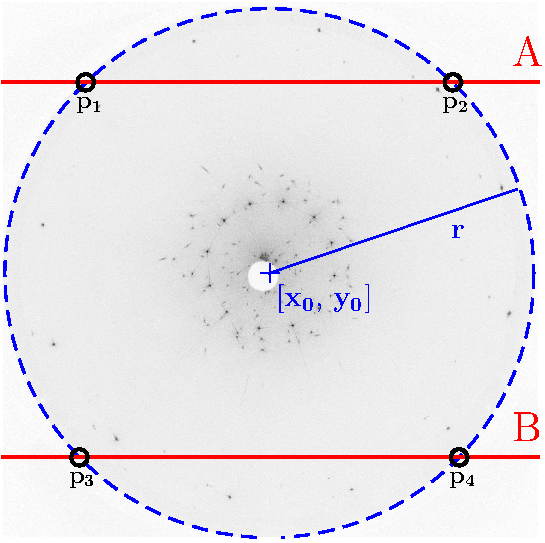
\includegraphics[width=\textwidth]{circleFit.pdf}
    \end{minipage}
    \begin{minipage}[c]{0.48\textwidth}
        \centering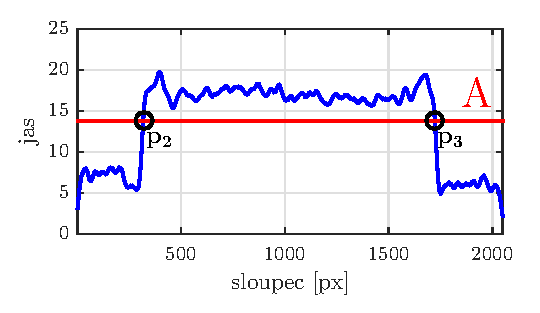
\includegraphics[width=\textwidth,height = 0.5\textwidth]{brigCutA.eps}\\
        
        \centering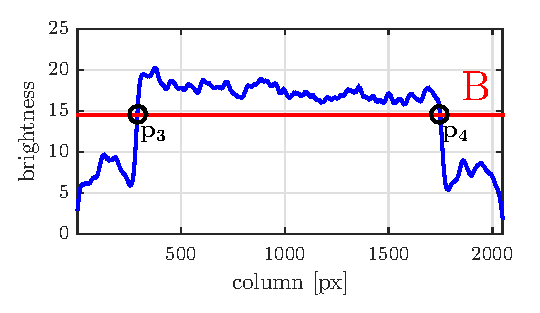
\includegraphics[width=\textwidth,height = 0.5\textwidth]{brigCutB.eps}
    \end{minipage}
    \\
        \caption[Detekce okolí stínítka.]{Jasové řezy \textit{A} a \textit{B}. Detekujeme body na kružnici $p_1$, $p_2$, $p_3$ a $p_4$. Metodou nejmenších čtverců odhadneme parametry kružnice $x_0$, $y_0$ a $R$.}
        \label{fig:CircleFit}
\end{figure}

Body na kružnici nalezeme pomocí sečen. Sečny sestrojíme ve dvou řádcích snímku. %a nalezneme sloupce, ve kterých protínáme kružnici.  
Sestrojením sečny získáme jasový řez v celé šířce snímku. Fotonový šum jasu vyfiltrujeme konvolucí s Gaussovým filtrem. Velikost filtru volíme \SI{21}{\px} a směrodatnou odchylku $\sigma = $ \SI{20}{\px}. 

Vyfiltrovaný jas oddělíme prahem. Práh určuje střední hodnota jasu v daném řezu. Nalezneme sloupce, kde je jas vyšší než prahové hodnota. Sloupec s minimálním resp. maximálním počtem pixelů určuje bod na kružnici.  

Každá sečna protíná kružnici ve dvou bodech, proto dostaneme celkem čtyři body na kružnici. Parametry kružnice určíme metodou nejmenších čtverců. 

Okolí stínítka poté definuje funkce 

\begin{equation}
	\left(x-x_0\right)^2 + \left(y-y_0\right)^2 > r^2\,.
	\label{eq:kruzniceOkoli}
	\end{equation}




\subsection{Pozadí snímku}
	V obraze nalezneme podstavec a okolí stínítka. Podstavec je specifický nízkou střední hodnotou jasu a jeho obraz je téměř ideální kruh. V seznamu MSER oblastí proto podstavec snadno nalezneme. Okolí stínítka již známe (kap. \ref{sec:okoliStinitka}).
	
	Velikost jasu v okolí stínítka nastavíme na hodnotu odvíjející se od střední hodnoty jasu snímku. Jas pixelů v oblasti podstavce nastavíme na střední hodnotu jasu pixelů v blízkém okolí podstavce.  
	
	Pozadí následně určíme konvolucí s Gaussovým filtrem. Tento filtr ignoruje vysoké změny jasu v obraze. Parametry filtru: velikost masky - \SI{201}{\px}, směrodatná odchylka $\sigma = $ \SI{201}{\px}.
	
	Samotná konvoluce s tímto filtrem by s použitím standardní funkce \textit{conv2} byla příliš časově náročná, proto konvoluci provádíme efektivnějším způsobem, který využívá rozkladu masky filtru na singulární čísla.
	
\begin{figure}[htbp]
    \centering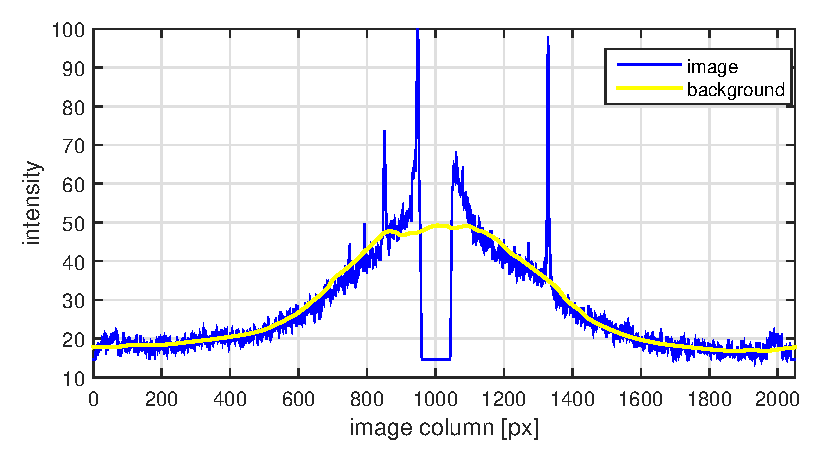
\includegraphics[width=.9\textwidth]{image_rust2.eps}
     \caption[Filtrace pozadí.]{Filtrace pozadí v HDR snímku znázorněná v řádku obrazu protínajícím obraz podstavce na kámen.}
        \label{fig:pozadi}
\end{figure}
	     
	     \newpage
\subsection{Odstranění nežádoucích detekcí}

Výstupem detektoru je soubor MSER oblastí. U výrazné světelné stopy dostaneme data ve formě pyramidy MSER oblastí podle jednotlivých úrovní intenzity. 

MSER detektor však najde nejen oblasti s výrazně vyšší intenzitou, ale i oblasti s nižší intenzitou než okolí. Ty je třeba vyřadit, protože nereprezentují světelnou stopu, kterou hledáme. 

K odstranění nežádoucích detekcí použijeme následující postup. 

\begin{enumerate}
\item Od filtrovaného snímku odečteme pozadí.

\item Ve vzniklém snímku vypočítáme střední hodnotu jasu MSER oblastí. 

\item Pokud je střední hodnota jasu záporná, MSER oblast odstraníme.  
\end{enumerate}

\section{Výsledek detekce}
Výsledky detekce světelných stop v obraze navrženého detektoru jsou srovnatelné s výstupem programu \textit{Source Extractor} \cite{SEXarticle}. Použití MSER detektoru je oproti \cite{SEXarticle} výhodné v tom, že přesně vymezuje oblast v obraze, kde se stopa nachází. Toho využíváme k určení parametrů svazků (kapitola \ref{sec:beam parameters} a \ref{sec:tails}). Ukázka detekce je na obrázku .

\begin{figure}[h!]
\centering
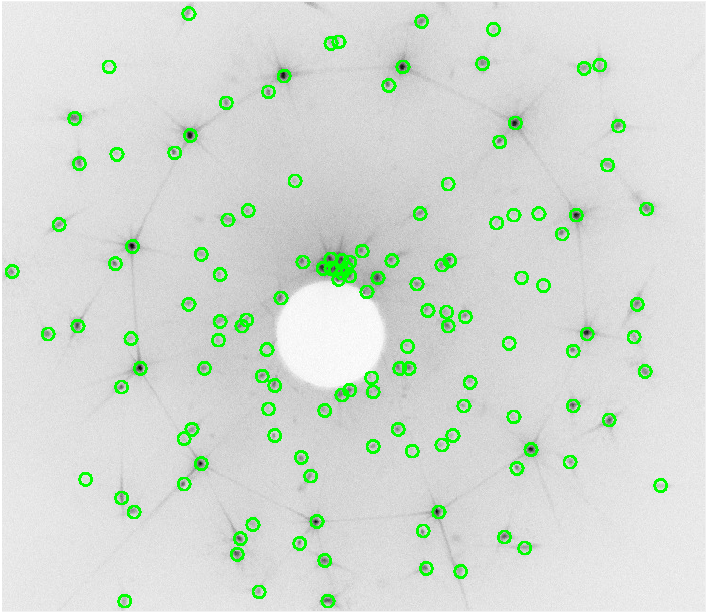
\includegraphics[width = 0.85\textwidth]{detekceVysledek.pdf}
\caption[Ukázka detekce světelných stop v obraze.]{Ukázka detekce světelných stop v obraze. }
\label{fig: podstavec}
\end{figure}

 	      

\section{Určení parametrů svazku}
\label{sec:beam parameters}
Základním parametrem svazku je směr šíření popsaný azimutem a elevací. Směr šíření svazku snadno dopočítáme, pokud nalezneme jeho obraz. Pozici světelné stopy v obraze lze určit jako polohu pixelu s maximálním jasem v detekované oblasti. Šum v obraze ale situaci komplikuje. Z obr. \ref{fig:rezy} ale vidíme, že pixel s maximálním jasem nemusí vždy určovat pozici dopadu a navíc nemusí být unikátním maximem.

Velikost obrazu měřeného svazku závisí především na jeho rozbíhavosti. Svazek od opuštění kamene do dopadu na stínítko vlivem rozbíhavosti několikanásobně zvýší svoji plochu, a proto nejsme schopni určit plochu svazku. Ze stejného důvodu nemůžeme u měřeného svazku odečítat intenzitu. Za předpokladu, že rozbíhavost svazků není příliš velká se zachová zářivý tok svazku a ten můžeme po odečtení pozadí vypočítat. %Je zřejmé, že část zářivého toku svazku se ztratí v pozadí snímku.   

V okolí obrazu svazků jsou patrné ocásky. Detekce ocásků a jejich klasifikace je popsána v samostatné kapitole \ref{sec:tails}.

Rozbíhavost svazků nemusí být ve všech směrech stejná. Na stínítku tak svazky tvoří stopy různých tvarů. Tvar stopy definujeme pomocí 3 parametrů.

\subsection{Základní parametry}

Máme detekované MSER oblasti. Nalezneme průniky oblastí a sestavíme stromovou strukturu. Kořenem stromu bude oblast s největší plochou a postupně se budou přidávat oblasti menší. Princip je patrný z 2D pohledu na prahovací úrovně MSER detektoru v obr. \ref{fig:gaussIntersection}, kde vidíme i princip tvorby stromu. Výsledkem bude řada stromů s různým počtem listů. Počet všech listů určuje počet detekovaných stop v obraze.

\begin{figure}[htbp]
    \centering
	\begin{minipage}[c]{0.78 \textwidth}
    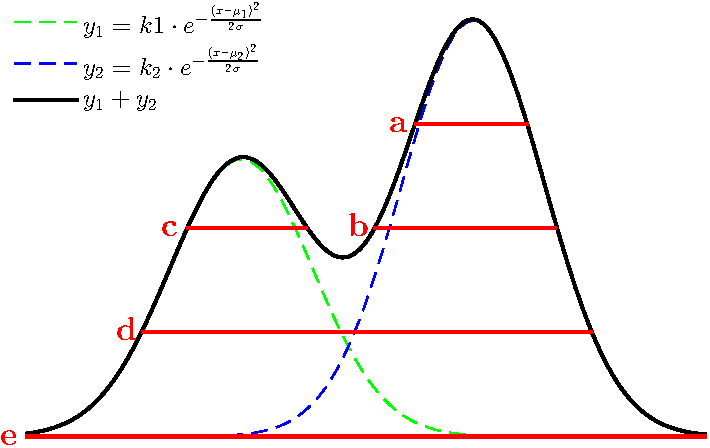
\includegraphics[width=0.95\textwidth]{gaussIntersection.pdf}
    \end{minipage}
    \begin{minipage}[c]{0.16 \textwidth}
    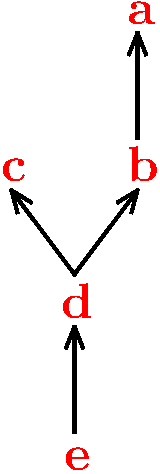
\includegraphics[width=0.95\textwidth]{treeGauss.pdf}
    \end{minipage}
    
    
     \caption[]{Ilustrace překrytí stop v 2D řezu. Výsledná charakteristika je součtem dvou Gaussových funkcí. Červeně jsou zakresleny prahovací úrovně MSER detektoru. Vlevo vidíme stromovou strukturu MSER oblastí a-f. Kořenem stromu je vrstva \textbf{e}. Vrstva \textbf{d} je jediný vnitřní uzel stromu. Listy představují vrstvy \textbf{c} a \textbf{a}. Důležité jsou podstromy \textbf{e}$\rightarrow$\textbf{d}, \textbf{c}, \textbf{b}$\rightarrow$\textbf{a}.}
        \label{fig:gaussIntersection}
\end{figure}

Cíleně prohledáváme jednotlivé stromy a nalézáme uzly, ze kterých počítáme parametry svazků.

\begin{itemize}
	\item \textbf{Azimut a elevace} - Pozici dopadu světelného svazku určíme jako střed eliptické aproximace oblasti odpovídající listu stromu. Pomocí transformace z \cite{Drapela} získáme azimut a elevaci.
	
	\item \textbf{Zářivý tok} - 
	Od filtrovaného snímku odečteme pozadí (obr. \ref{fig:pozadi}) a získáme snímek, ze kterého budeme odečítat intenzitu pixelů. Algoritmus výpočtu zářivého toku je následující:
	\begin{enumerate}
	\item $t_0$ = původní strom; $i = 0$; $q = 0$; $n_0$ = počet listů v $t_0$;
	
	\item Ve stromu $t_i$ nalezneme podstromy $\tau_1,\dots,\tau_n$ maximální velikosti bez vnitřních uzlů stromu $t_i$ a obsahující jeden list stromu $t_i$.  
	
	\item Nalezneme kořeny $\xi_1,\dots,\xi_n$ podstromů $\tau_1,\dots,\tau_n$. Kořeny odpovídají oblastem s množinou pixelů $\mathbb{M}_{q+1},\dots,\mathbb{M}_{q+n}$.
	
	\item Pokud $i = 0$ vypočítáme zářivý tok 
	
	\begin{equation}
	\underset{{k = 1}}{\sum}
	\phi_{e_j} = \frac{\underset{k\in\mathbb{M}_j}{\sum}I_k}{N_j}\,,\hspace{2cm} j\in\lbrace1,\dots,n_0\rbrace
	\end{equation}
	kde $I_k$ je jas pixelu $k$ ve snímku a $N_j$ je počet pixelů v množině $\mathbb{M}_j$. Index $j$ odpovídá indexu stopy ve stromu $t_0$.\\
	
	Pokud $i > 0$ nalezneme množiny $\mathbb{P}_1,\dots,\mathbb{P}_n$. $\mathbb{P}_l$ je množina indexů listů, které jsou v $t_0$ potomkem uzlu $\xi_l$, kde $l\in {1,\dots,n}$. Zářivý tok stop upravíme.  
	 \begin{equation}
	\phi_{e_j} = \frac{\phi_{e_j}}{\underset{q\in \mathbb{P}_l}{\sum}\phi_{e_q}}\frac{\underset{{\lbrace k\in\mathbb{M}_{q+l}\cap\lbrace \mathbb{M}_1^c \cup \mathbb{M}_2^c \cup \dots \cup \mathbb{M}_q^c \rbrace\hspace{1.5mm}|\hspace{1.5mm} \lbrace1,2,\dots,q\rbrace = \mathbb{P}_l \rbrace}}{\sum} I_k}{N_{q+l}} + \phi_{e_j}\,.\hspace{0.5cm} j\in \mathbb{P}_l
	\end{equation}
	
	\item $i = i+1$; $q = q+n$;
	\item Pokud $n \neq 1$ odstraníme podstromy $\tau_1,\dots,\tau_n$ z grafu $t_{i-1}$, získáme strom  $t_i$ a opakujeme od kroku $2$. 
	
\end{enumerate}	
	\item \textbf{Tvar} -  Pro každou MSER oblast je určena elipsa, která uzavírá danou oblast. U této elipsy lze určit orientaci a velikost hlavních poloos. 
	
	Každé stopě odpovídá jeden list stromu. Nalezneme cestu $\mathcal{C}$, která je cestou od kořene k listu. 	
	
	Orientace je určena jako medián orientací elips všech MSER oblastí v cestě $\mathcal{C}$. Velikosti hlavních poloos jsou určeny podle MSER oblasti, která je uprostřed cesty $\mathcal{C}$.		
		
\end{itemize}

\newpage
\section{Detektor ocásků}
\label{sec:tails}
	Se znalostí směru a velikosti ocásků detekovaných svazků dostáváme nové informace, které nohou přispět k jejich správnému párování se svazky z matematického modelu kamene.
	
	Ve snímaném obraze nelze rozpoznat všechny vznikající ocásky, ale pouze ty s dostatečně velkou intenzitou.

	Princip detektoru ocásků zjednodušeně spočívá v převodu okolí stopy do polárních souřadnic (vzdálenost $\rho$ a směrový úhel $\phi$) a nalezení směru, kde je patrný výrazný vzestup intenzity jasu oproti okolí. Zvýšená intenzita jasu je typicky důsledkem přítomnosti ocásku v obraze. 
	
	Abychom mohli rozvinout okolí stopy do polárního grafu, musíme si být vědomi překážek komplikující detekci ocásků.
	  
	 \begin{itemize}	 	
	 	\item V blízkém okolí jedné stopy se může nacházet další stopa. V polárním grafu se tato blízká stopa jeví jako ocásek a dochází k falešné detekci.	
	 	\item Různé stopy a ocásky mají v obraze různou velikost. Je třeba efektivně určovat vzdálenost $\rho$ do které budeme převádět okolí stopy do polárního grafu. Pokud zvolíme malé $\rho$, nepokryjeme oblast, kde se vyskytují ocásky. Příliš velké $\rho$ zvýší časovou náročnost výpočtu.   	
	 	\item Polární graf je citlivý na určení pozice dopadu svazku. 
	\end{itemize}
	
	Elegantní řešení přináší použití MSER detektoru, pomocí něhož získáme vymezení oblasti a tím i vzdálenosti $\rho$, kde se stopa i s ocásky nachází. Se znalostí oblastí náležící jednotlivým stopám jsme schopni od sebe stopy částečně oddělit a redukovat množství falešných detekcí. Na druhou stranu sousední stopa může ležet na pozici ocásku a odstraněním sousední stopy odstraníme současně i ocásek, který prozatím nejsme schopni v případě překrytí oddělit. Vzhledem k rozmanitosti stop, co do velikosti, intenzity, množství a tvaru ocásků apod. není jednoduché stopu matematicky modelovat. Pokud by se podařilo vytvořit dostatečně přesný kompaktní model stopy, je možné uvažovat o situaci, kdy budeme schopni od sebe separovat překrývající se stopy a ocásky. 
	
 Pro znázornění postupu a mezivýsledků jsme si vybrali laserovou stopu (obr. \ref{fig:mark_tail}, \ref{fig:mark_tail2}), která v obraze nekoliduje s další výraznou stopu. Zvolená stopa vznikla dopadem svazku třídy \textbf{6C}. V obraze jsou patrné čtyři ocásky různé intenzity. 
	

	\begin{figure}[h!]
	\centering
	\begin{minipage}[c]{0.35\textwidth}
	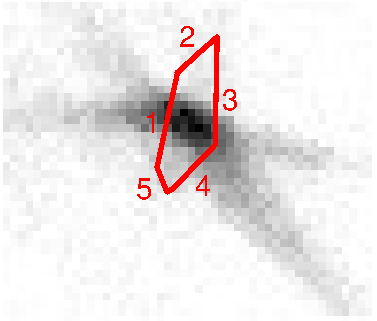
\includegraphics[width=\textwidth]{figures/tail007.pdf}
	\end{minipage}
	\begin{minipage}[c]{0.35\textwidth}
	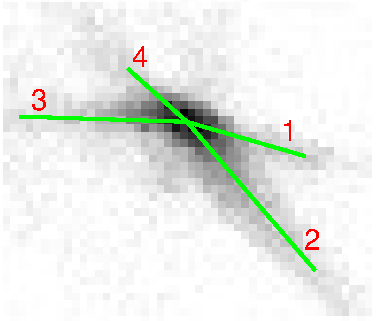
\includegraphics[width=\textwidth]{figures/tail008.pdf}
	\end{minipage}
	
	\caption[Detektor ocásků - stopa v obraze.]{Vybraná světelná stopa k ilustraci algoritmu k detekci ocásků. Stopa vznikla dopadem svazku třídy \textbf{6C} na stínítko. Vlevo: 70$\times$ zvětšený polygon simulovaného svazku. Polygon je ohraničen hranami kamene. Na hranách vznikají ocásky. Vpravo: ocásky detekované v obraze. Číslování ocásků odpovídá číslování hran na obrázku vlevo, tzn. na hraně 1 vzniká ocásek 1 atd.}
	\label{fig:mark_tail}
	\end{figure}
	



	\begin{figure}[h!]
	\centering
	\begin{minipage}[c]{0.4\textwidth}
	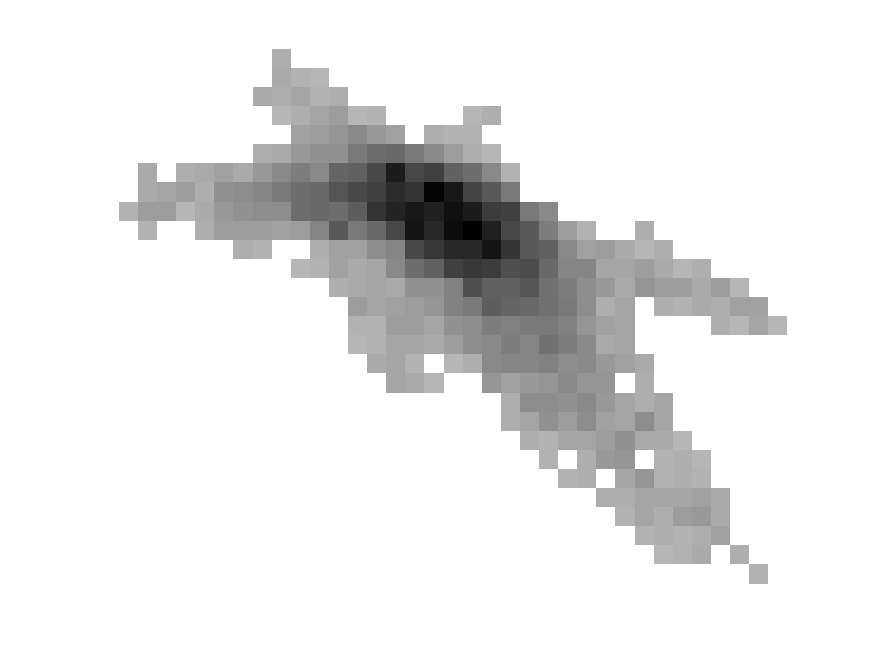
\includegraphics[width=\textwidth]{figures/tailex01.pdf}
	\end{minipage}
	\begin{minipage}[c]{0.4\textwidth}
	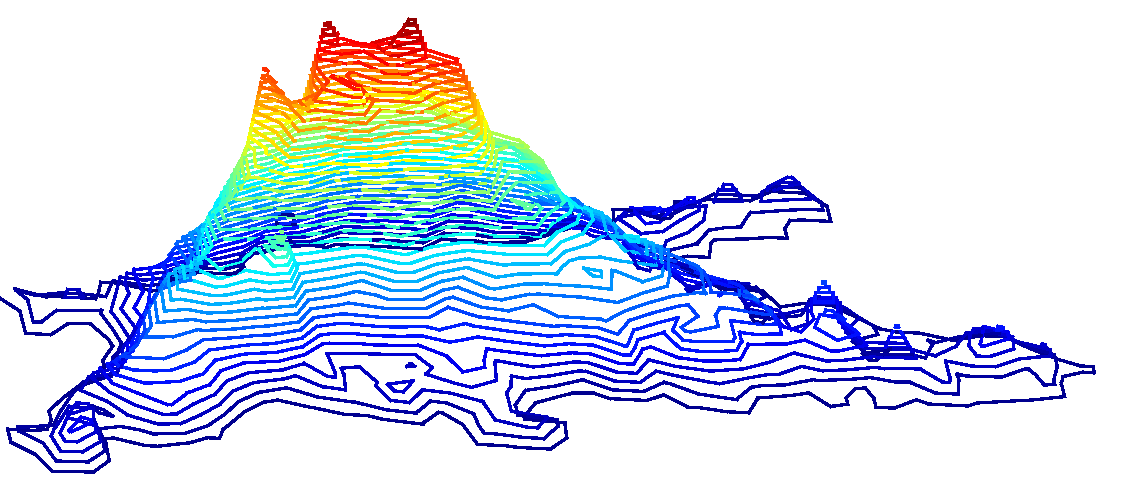
\includegraphics[width=\textwidth]{figures/tailex02.pdf}
	\end{minipage}
	
	\caption[Detektor ocásků - detekce stopy.]{Stejná světelná stopa jako na obr. \ref{fig:mark_tail}. Vpravo: detekovaná MSER oblast. Vlevo: 3D pohled na stopu.}
	\label{fig:mark_tail2}
	\end{figure}


\paragraph{Jednotlivé kroky algoritmu}

	\begin{itemize}
	\item Vybereme stopu, u které chceme identifikovat ocásky a ze snímku vybereme oblast (obr.\ref{fig:mark_tail}), která náleží zkoumané stopě. 
	
	\item U vybrané oblasti odečteme intenzitu okolí $I_o$ a vypočítáme střední hodnotu intenzity $I_m$. Intenzitu pixelů omezíme maximálně na intenzitu o velikosti $2\cdot I_m$ a potom ke všem pixelům přičteme intenzitu $I_m$. Důvodem tohoto kroku je snaha odstranit nežádoucí vlastnosti velkého šumu v hodnotách intenzity v blízkém okolí těžiště stopy a také to, že se chceme zvětšit relativní příspěvek pixelů s nižší intenzitou do součtového kritéria \ref{eq:Isuma}.   
	
	\item Oblast převedeme do polárních souřadnic ($\rho$, $\phi$). Intenzitu $I_{pol}$ v polárním grafu $I_{pol} = f(\phi,\rho)$ určujeme pomocí bipolární interpolace, která pro větší efektivitu vynechává oblasti mimo oblast stopy, kde $I_{pol} = 0$. Důležitým parametrem při interpolaci je velikost vzorkování $f_{\phi}$ úhlu $\phi$ resp. vzorkování $f_{\rho}$ vzdálenosti $\rho$ . Experimentálně jsme zvolili $f_{\phi} = \SI{3}{\degree}$ a $f_{\rho} = \SI{1}{\px}$. Interpolaci počítáme v intervalech  $\phi \in \left\langle 0,2\pi \right\rangle$ a $\rho \in \left\langle 1,\rho_{max} \right\rangle$, kde $\phi_{max}$ je maximální vzdálenost všech pixelů v oblasti stopy od její pozice.  
	
	\begin{figure}[htps]
    \centering
    \begin{minipage}[c]{0.48\textwidth}
        \centering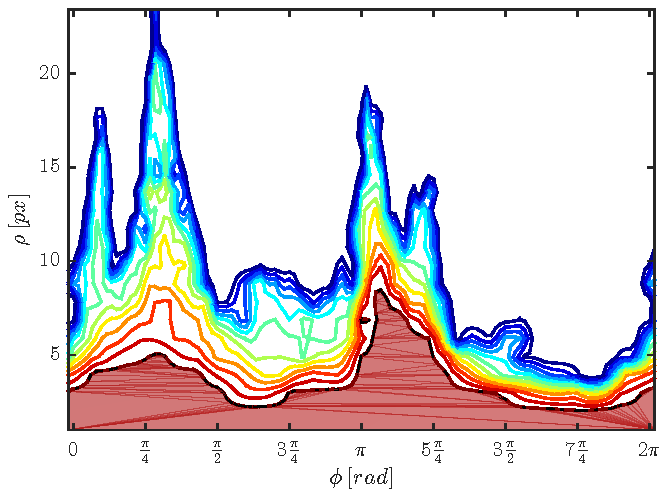
\includegraphics[width=\textwidth]{tailex03.pdf}
    \end{minipage}
    \begin{minipage}[c]{0.48\textwidth}
        \centering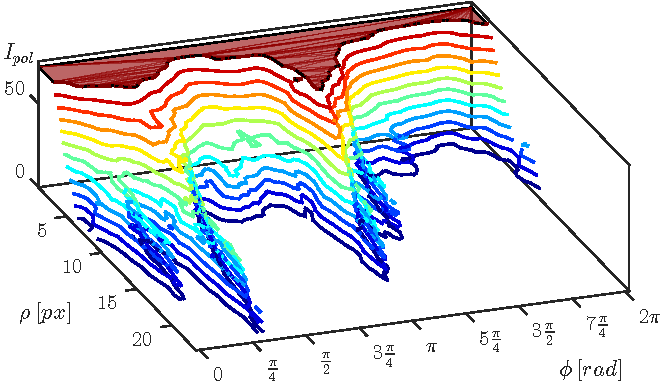
\includegraphics[width=\textwidth]{tailex04.pdf}
    \end{minipage}
    \\
        \caption[Detektor ocásků - polární graf.]{Dva pohledy na intenzitu okolí stopy převedené do polárního grafu $I_{pol}$ zobrazené pomocí vrstevnic.}
        \label{Detekce}
\end{figure}
	
	\item Provedeme součet intenzit $I_{pol}$ pro jednotlivé úhly $\phi$ od minimální do maximální vzdálenosti $\rho$ a získáme závislost $I_\phi = f(\phi)$, kde  
	
	\begin{equation}
	I_{\phi_i} = \sum_{j = 1}^{\rho_{max}} I_{pol}\left(i,j\right)\,. \hspace*{2cm} i \in \left\lbrace 0, \frac{3}{180}\pi, \dots \,,2\pi \right\rbrace
	\label{eq:Isuma}
	\end{equation}
	Následně na $I_{\phi}$ aplikujeme kubickou interpolaci sousedních hodnot s $5$krát citlivějším vzorkováním $f_{\phi_2} = \frac{f_{\phi}}{5}$ a rozšíříme rozsah $\phi$ na $\phi \in \left\langle -\frac{\pi}{2},\frac{5}{2}\pi \right\rangle$. 
	
	\item Graf závislosti $I_\phi = f(\phi)$ filtrujeme konvolucí s Gaussovou funkcí $g(x)$ se směrodatnou odchylkou $\sigma = \SI{1.2}{\degree}$ a získáme referenční závislost $I_{filt}$.
	
	\begin{equation}
		g(x) = \frac{1}{\sqrt{2\pi} \cdot \sigma}e^{-\frac{x^2}{2\sigma^2}}\,.
	\end{equation}
	
	\begin{figure}[htbp]
    \centering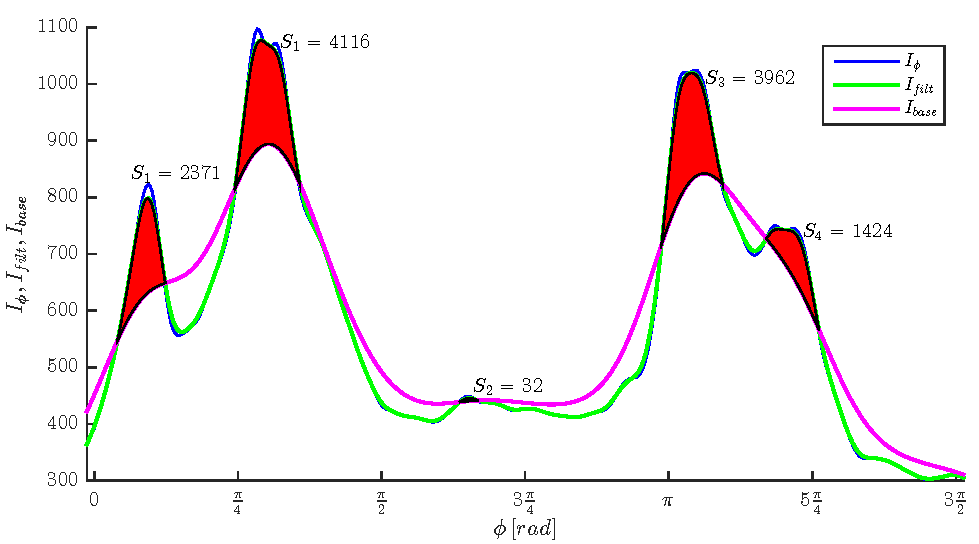
\includegraphics[width=\textwidth]{figures/tailex05.pdf}
     \caption[Detekce ocásků - zpracování polárního grafu.]{Grafické vysvětlení funkce algoritmu pro detekci ocásků. }
    \label{fig:tailSumGraph}
	\end{figure}
	
	\item Na graf $I_{filt}$ následně opakovaně aplikujeme konvoluci, tentokrát s Gaussovou funkcí $g(x)$ s vyšší směrodatnou odchylkou $\sigma = \SI{4.8}{\degree}$, abychom získali základnu $I_{base}$, kterou budeme porovnávat se signálem $I_{filt}$.
	
	\item Nalezneme souvislé oblasti $\mathcal{R}_1, \dots , \mathcal{R}_n$, kde graf $I_{filt}$ má větší hodnotu než $I_{base}$ a sečteme rozdíly $I_{filt}$ a $I_{base}$ v jednotlivých vzorcích. Velikost součtu $S_1, \dots , S_n$ závisí na vzorkovací frekvenci $f_{\phi_2}$.
	
	\begin{equation}
	S_i = \sum_{\phi_j \colon \phi_j \in \mathcal{R}_i}I_{filt}(\phi_j)-I_{base}(\phi_j)\,. \hspace*{2cm} i \in \left\lbrace 1, 2, \dots \,, n \right\rbrace
	\label{eq:Rsuma}
	\end{equation}
	
	\item Za ocásek uvažujeme oblast $\mathcal{R}_i$, kde je součet $S_i$ větší než prahovací úroveň $s_{th}$ (pro $f_{\phi_2}$ je $s_{th} = 500$). Směr ocásku $\varphi$ je určen jako úhel, ve kterém je graf $I_{filt}$ v dané oblasti maximální a velikost ocásku $\varrho_i$ určuje $\rho_{max}$ a poměr součtu $S_i$ k maximálnímu v pro danou stopu.  
	
	\begin{equation}
	\varphi_i = \argmax_{\phi_j \colon \phi_j \in \mathcal{R}_i}I_{filt}(\phi_j) \,, \hspace{1cm} \varrho_i = \frac{S_i}{\max_{j \in 1,\dots , n}S_j}\rho_{max}\,.
	\label{eq:tail_params}
	\end{equation}
		
	\begin{figure}[htbp]
    \centering
    \begin{minipage}[c]{0.48\textwidth}
        \centering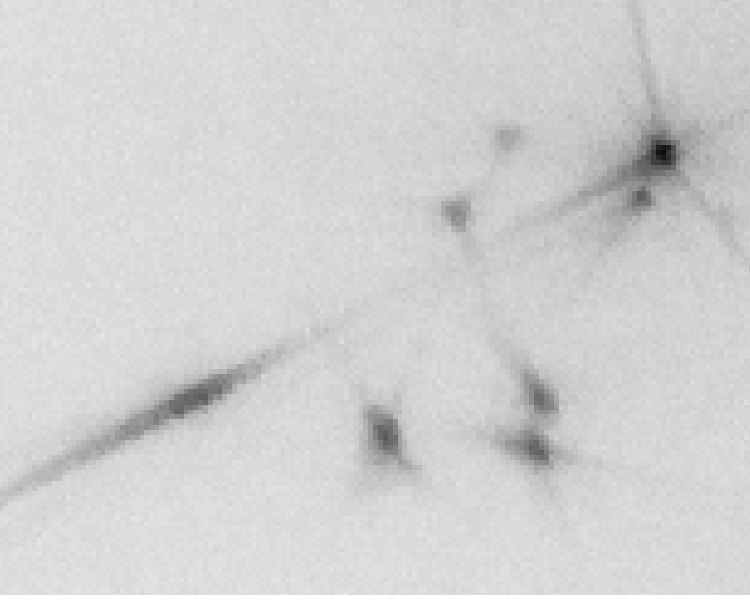
\includegraphics[width=.98\textwidth]{tail01.pdf}
    \end{minipage}
    \begin{minipage}[c]{0.48\textwidth}
        \centering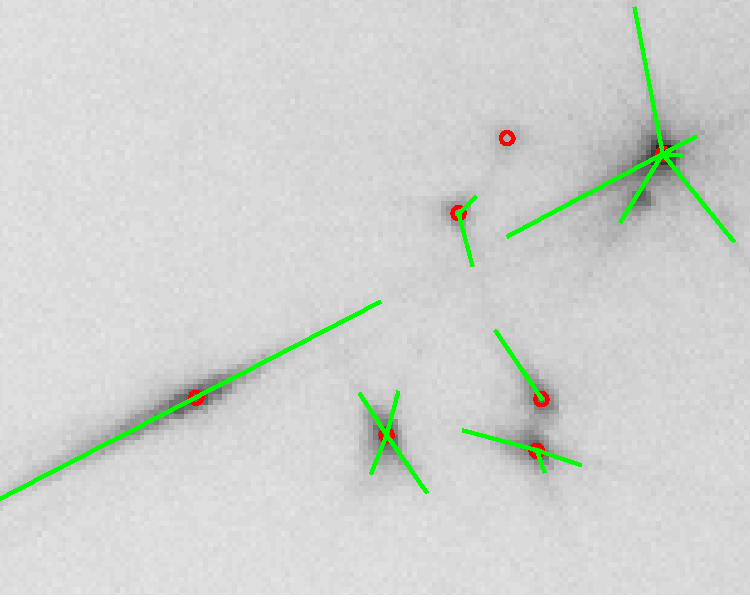
\includegraphics[width=.98\textwidth]{tail02.pdf}
    \end{minipage}
    \\
        \caption[Detektor ocásků - příklad detekce.]{Ukázka funkce detektoru ocásků na vybraném vzorku z obrazu. }
        \label{Detekce}
\end{figure}
	
\end{itemize}	   
	
	

%\section{MSER detector configuration parameter list}	
%	Here is a list of the configuration parameters used for beam detection setting. All of them can be used with their default values. This description of the parameters can be usefull for understanding the algorithm or debugging.
%	
%\begin{center}
%
%
%\begin{tabular}{l|l|p{8cm}}
%    \textbf{Name} 		& \textbf{Default} & \textbf{Description} \\ \hline \hline 
%    \textit{BackgroundFilt}	    	& $201$ 	& Size of Gaussian filter mask used for background estimation. \textit{Sigma} of mask is equal to \textit{BackgroundFilt} \\ \hline
%    \textit{BackgroundKMean}    	& $0.15$	& $BackgroundKMean \times mean(image)$ is added to background estimation. \\ \hline
%    \textit{ComputeAllLayers}   	& $1$		& $1$ - Divide all layers in marks variable calculation. $0$ - Calculate only with upper layers. \\ \hline
%    \textit{ComputeTails}   		& $ 1 $		& $1$ - Tails of marks are computed. It takes some time. $0$ - No tails. Faster.\\ \hline    
%    \textit{CleanerAxisRatio}   	& $ 10 $	& MSER regions with upper axis ratio are deleted. \\ \hline
%    \textit{CleanerFilterSigma}  	& $ 5 $		& \textit{Sigma} of filter mask in image blurring. \\ \hline
%    \textit{CleanerFilterSize}   	& $ 31 $	& Size of filter mask in image blurring.\\ \hline
%	\textit{CleanerMean}    		& $ 0.035 $ & Regions with peak where difference of mean of surrounding
%intensity is lower than $CleanerMean \times mean(image)$ are deleted. \\ \hline
%    \textit{CleanerSumWide} 		& $ 5 $		& Size of surrounding in cleaning process.  \\ \hline
%    \textit{FilterSigma}    		& $ 0.7 $	& \textit{Sigma} of niose reducing filter mask. \\ \hline
%    \textit{FilterSize} 			& $ 3 $		& \textit{Size} of niose reducing filter mask.\\ \hline 
%    \textit{MSERMaxAreaVar} 		& $ 0.9 $	& This value specifies the step size between intensity threshold levels used in selecting extremal regions while testing for their stability. Decrease this value to return more regions.\\ \hline
%    \textit{MSERRegion} 			&$[2\,,\, 14000]$& Two-element vector, [minArea maxArea], which specifies the size of the regions in pixels. This value allows the selection of regions containing pixels between minArea and maxArea, inclusive.\\ \hline
%    \textit{MSERThresh} 			& $ 1.2 $	& Increase this value to return a greater number of regions at the cost of their stability. Stable regions are very similar in size over varying intensity thresholds.\\ \hline
%    \textit{SurroundThres}   		& $ 0.8 $	& Multiple of $mean(image)$ where surrounding intensity is moved.   \\ 
%\end{tabular}
%
%\end{center}

\clearpage
\part{Klasifikace příznaků}

Nalézt korespondující dvojice měřených a referenčních svazků pouze pomocí směru svazků je prakticky nemožné. Víme, že u měřených svazků můžeme kromě směru určit zářivý tok a detekovat ocásky (kapitola \ref{sec:beam parameters}).   

Prozkoumáme parametry referenčních a měřených svazků s cílem definovat závislost parametrů pomocí jednoduché funkce. Nalezení závislosti parametrů zjednoduší úlohu korespondence svazků.  


\section{Ground truth}

Abychom mohli hledat závislosti mezi parametry měřených a referenčních svazků, potřebujeme získat data  s korespondujícími svazky. Toho dosáhneme tak, že ručně upravujeme množinu korespondencí a optimalizujeme náklon faset. Proces ručního přiřazování svazků ukončíme, když nalezneme optimální náklon faset, který zajišťuje maximální shodu měřených a referenčních svazků. Tyto korespondence považujeme za správné.    

Ručně určené korespondence označujeme výrazem "\textit{ground truth}" podobně jako v oblasti strojového učení, kde slouží jako přesná data v trénovací množině pro určení statistických modelů. Použití výrazu "\textit{ground truth}" je ovšem v našem případě sporné, neboť určení množiny korespondencí závisí na osobě, která tato úlohu provádí. To, co v našem případě označujeme jako "\textit{ground truth}", je množina, o které se domníváme, že by měla obsahovat správné korespondence svazků, ale v našem případě nemůžeme s naprostou jistotou tvrdit, že tomu tak je. 

\section{Změna zářivého toku se změnou parametrů kamene}
\label{sec: zmena_tok }

	Chceme zjistit, jak je zářivý tok svazků závislý na změně parametrů faset. 

	Máme k dispozici 27 snímků, které zachycují 9 různých kamenů typu \textit{viva12}. Při určení "\textit{ground truth}" jsme zároveň nalezli optimální matematické modely kamenů. Vezmeme si postupně každý s těchto modelů a měníme náklon normály vybrané fasety o jeden stupeň ve čtyřech kolmých směrech. Nakonec normálu vrátíme zpět na původní hodnotu. Takto nakloníme normály všech 14-ti faset kamene.
	
	Nakloněním normály fasety vznikne nový model kamene. Pro tento model pomocí LADOKu  vyřešíme parametry svazků. Pokud se zářivý tok svazku od původního modelu změnil, zapamatujeme si jeho hodnotu. Pro jednotlivý svazek dostaneme vektor hodnot zářivého toku $\vv{\phi_e}$. 
	
	 Abychom mohli porovnat změnu zářivého toku, který se může u svazků řádově lišit, vyjádříme změnu toku pomocí variačního koeficientu $c_v$. Variační koeficient je výsledkem podílu směrodatné odchylky a střední hodnoty vektoru $\vv{\phi_e}$. 
	 
	 \begin{equation}	 
	 c_v = \frac{\sigma(\vv{\phi}_e)}{E(\vv{\phi}_e)}\,. 
	 \end{equation}
	 
Určíme variační koeficient všech referenčních svazků se známými korespondujícími svazky a výsledek zaneseme do histogramu \ref{fig: flux_var_coeff}. V histogramu vidíme, že existuje nezanedbatelný počet svazků, pro které změna náklonu fasety o \SI{1}{\degree} znamená změnu zářivého toku o více než polovinu původní hodnoty. Je zřejmé, že obdobně se bude měnit zářivý tok svazků při posunu fasety. 

 Výsledek naznačuje, že nebude snadné nalézt funkci, která by definovala vztah mezi zářivým tokem referenčních a měřených svazků.  

\begin{figure}[htps]
\centering
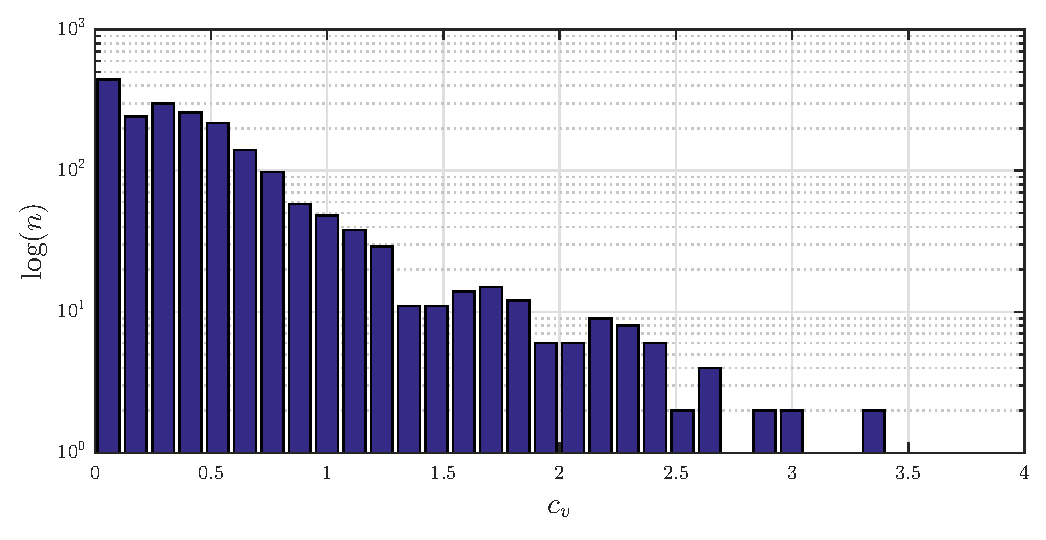
\includegraphics[width = \textwidth]{flux_var_coeff.eps}
\caption{Histogram variačního koeficientu zářivého toku svazků pro data z 27 snímků kamene \textit{viva12}.}
\label{fig: flux_var_coeff}
\end{figure}



\section{Závislost zářivého toku}
	Broušený kámen je ozářen laserovým svazkem o vlnové délce \SI{670}{\nano\metre}. Při průchodu světelného svazku kamenem se část záření absorbuje a přemění se na teplo. Absorpce záření závisí na odstínu kamene, proto si vybereme kameny stejného odstínu. V našem případě zvolíme odstín \textit{Hyacint}, který se vyznačuje nízkou absorpcí zdrojového svazku. 
	
	Korespondující svazky jsme určili pro 4 kameny odstínu \textit{Hyacint}, kde každý svazek byl 3$\times$ s různou rotací umístěn do měřicí soustavy. S korespondencemi z 12 snímků pracujeme jako s celkem a dostaneme množinu uspořádaných dvojic měřených a referenčních svazů. 
	
	Měřené svazky charakterizuje zářivý tok $\vv{\phi}_{e_m}$ a referenční svazky zářivý tok $\vv{\phi}_{e_r}$. Cílem je nalézt funkci $h$, pro kterou
	
	\begin{equation}	
		\phi_{e_r} = h \left( \phi_{e_m} \right) \,.
		\label{eq: fi_fi}
	\end{equation}

Abychom mohli porovnat data z více měření, vyjádříme si zářivý tok měřených svazků jako jejich poměr ku součtu zářivého toku všech měřených svazků v jednotlivém snímku. 

Závislost $\phi_{e_r} =  f\left( \phi_{e_m} \right)$ vyneseme do grafu \ref{fig: flux_depend2}, kde jsou vykresleny pouze svazky s variačním koeficientem $c_v$ menším než $0.5$. Do grafu zároveň zakreslíme hranice $\mathbf{b_0}$ a $\mathbf{b_1}$ vymezující oblast, kde se nachází většina svazků.

  Výsledek není příliš optimistický. Data v grafu jsou příliš rozptýlena na to, abychom mohli nalézt spolehlivou funkci popisující závislost \ref{eq: fi_fi}. Důvodů může být hned několik. 

Víme, že v modelu kamene nejsou postihnuty všechny skutečnosti ovlivňující velikost zářivého toku stop. Můžeme zmínit například to, že v modelu není zahrnuta čistota materiálu, která nemusí a prakticky ani není v celém materiálu konstantní. Nedokonalé proleštění fasety ovlivňuje rozptylové parametry světelného svazku. Změna parametrů fasety vede ke změně plochy fasety, tedy i ke změně plochy svazku, který je omezen hranou této fasety. Malá změna parametrů fasety může vést k velké změně zářivého toku svazku, což jsme si ukázali v kapitole \ref{sec: zmena_tok }. Tyto a další vlastnosti v konečném důsledku vyústí v chybu údaje na y-ové ose grafu \ref{fig: flux_depend2}.

Na druhé straně musíme počítat s nejistotou určení zářivého toku detekovaných svazků vznikající při extrakci parametrů svazků z obrazu. Mezi zásadní problémy patří šum, překrývání stop, difuzní odrazivost svazků či odhad pozadí snímku.  

\begin{figure}[htps]
\centering
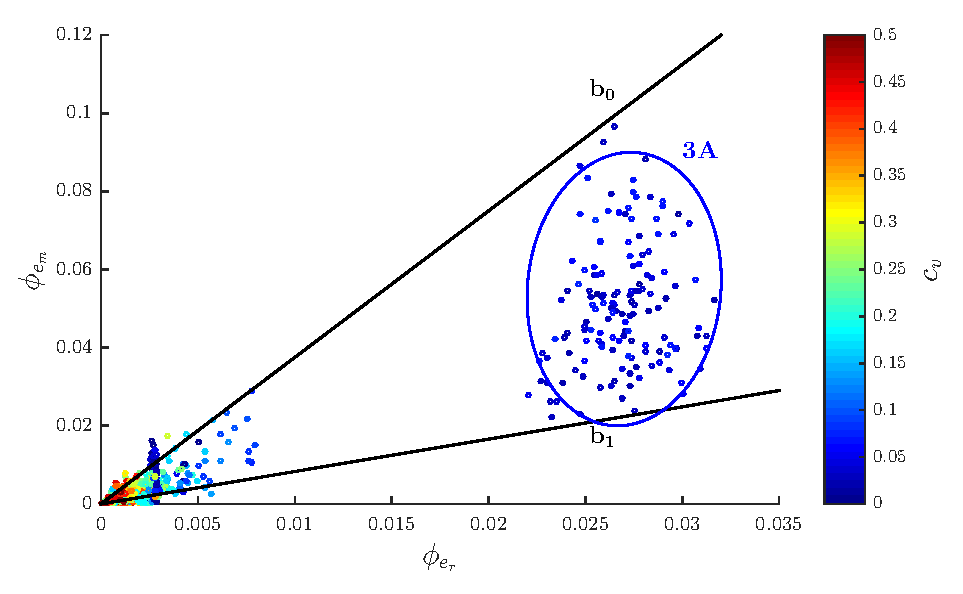
\includegraphics[width = 0.8\textwidth]{flux_depend2.eps}
\caption{Závislost zářivého toku referenčních svazků na velikosti zářivého toku měřených svazků. Zobrazeny jsou pouze svazky s variačním koeficientem zářivého toku větším než $0.5$. Zakresleny jsou vymezovací hranice $\mathbf{b_0}$ a $\mathbf{b_1}$. Výsledky pro odstín \textit{Hyacint}.}
\label{fig: flux_depend2}
\end{figure}

\begin{figure}[htps]
\centering
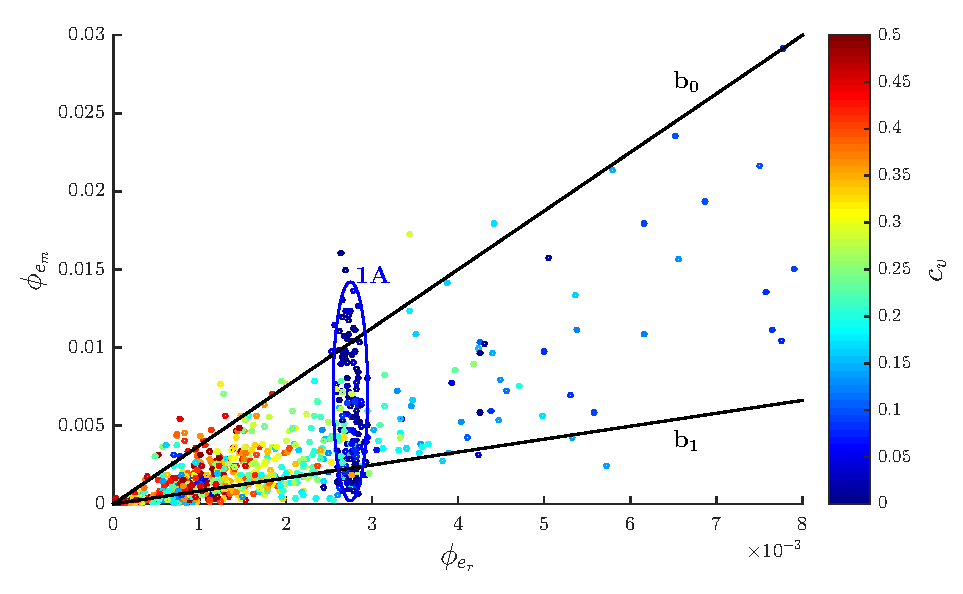
\includegraphics[width = 0.8\textwidth]{flux_depend1.eps}
\caption{Detail obrázku \ref{fig: flux_depend2}. Vynechány jsou svazky třídy \textbf{3A}.}
\label{fig: flux_depend1}
\end{figure}


Ve grafu \ref{fig: flux_depend2} jsou patrné shluky bodů, které přesto, že mají referenční zářivý tok podobné velikosti se velikost detekovaného zářivého toku znatelně liší. Při detailnějším pohledu zjistíme, že se jedná o stopy třídy (\textbf{1A} a \textbf{3A}). Tyto svazky se navíc vyznačují téměř nulovým variačním koeficientem zářivého toku. Pro třídu \textbf{1A} můžeme velké odchylky vysvětlit tím, že povrch kamene byl až matný a  odrážel tak více světla, než jsme očekávali. 

\section{Závislost parametrů ocásků}

	Zajímáme se to, jak může přispět znalost ocásků měřených s referenčních svazků k nalezení korespondující dvojice.  

  Korespondující ocásky nalezeme pomocí jednoduchého algoritmu založeného na podobnosti směru ocásků korespondujících stop a výsledek ručně upravíme. Máme k dispozici data korespondujících ocásků pro 25 snímků celkem deseti kamenů \textit{viva12}. 
	
	Ocásky parametrizujeme pomocí velikosti $\rho$ a směrového úhlu $\phi$. Z korespondujících ocásků získáme parametry měřených ocásků $\vv{\rho}_m$ a $\vv{\varphi}_m$ a k nim odpovídající parametry $\vv{\rho}_r$ a $\vv{\varphi}_r$.
	

\subsection{Směrový úhel}
 U směrového úhlu potřebujeme vědět, do jaké míry souhlasí směr měřeného a směr referenčního svazku. Vypočítáme rozdíl směrových úhlů $\Delta\vv{\phi}$ a vyneseme do grafu \ref{fig: tail_depend1} rozložení pravděpodobnosti.  
 
 \begin{equation}
 \Delta\vv{\phi} = \vv{\varphi}_m - \vv{\varphi}_r\,.
 \end{equation}
  
\begin{figure}[htps]
\centering
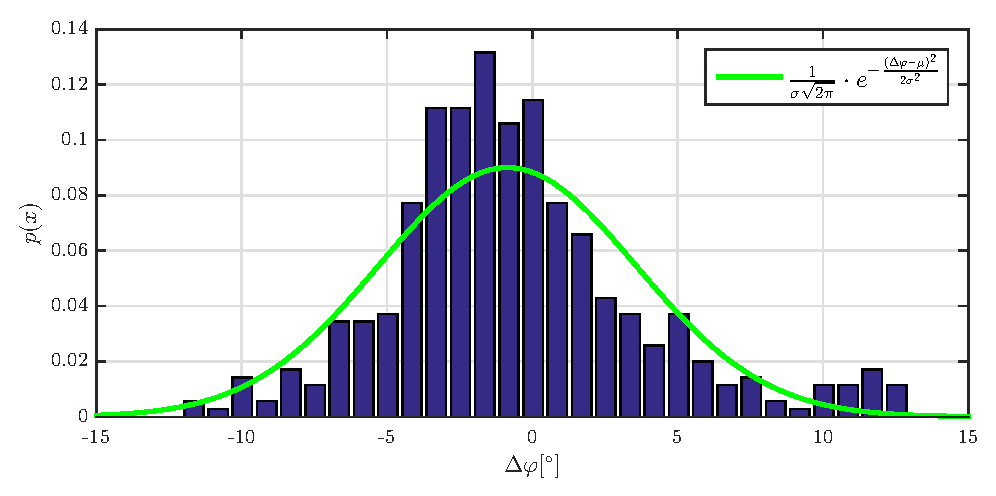
\includegraphics[width = 0.8\textwidth]{tails_gauss.eps}
\caption{Odhad pravděpodobnostní funkce rozdílu směrového úhlu mezi měřenými a referenčními ocásky. Aproximace Gaussovou křivkou s parametry $\sigma = $ \SI{4.43}{\degree} a $\mu = $ \SI{-0.86}{\degree}. }
\label{fig: tail_depend1}
\end{figure}

Pravděpodobnostní rozdělení na obr. \ref{fig: tail_depend1} lze aproximovat Gaussovu funkcí

\begin{equation}
f(\Delta\varphi) = \frac{1}{\sigma\sqrt{2\pi}}\cdot e^{-\frac{\left(\Delta\varphi - \mu\right)^2}{2\sigma^2}}\, 
\end{equation}
s rozptylem $\sigma =  $ \SI{4.43}{\degree} = \SI{0.077}{\radian} a střední hodnotou $\mu = $ \SI{-0.86}{\degree} = \SI{-0.15}{\radian}. Tato funkce může sloužit jako základ pro určení podobnostní ocásků.   

\subsection{Velikost}
	Vykreslili jsme si závislost velikosti referenčních ocásků na velikosti měřených ocásků. V grafu \ref{fig: tail_depend2} jsou pouze náhodně vybrané vzorky závislosti $\rho_r = f(\rho_m)$  , kde $\rho_m = \dfrac{\rho_m}{max{\vv{\rho}_m}}$. Naměřené velikosti ocásků se zdají být v souvislostí s velikostí referenčních ocásků takřka nahodilé. Nejsme schopni nalézt funkci $f$, která by popisovala závislost $\rho_r = f(\rho_m)$.
	
	\begin{figure}[htps]
\centering
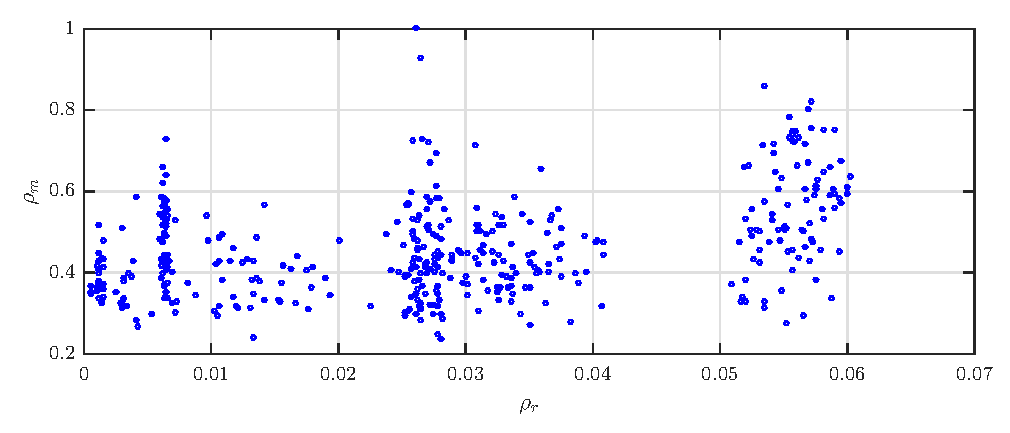
\includegraphics[width = 0.8\textwidth]{tails_rho.eps}
\caption{Závislost velikosti referenčních ocásků $\rho_r$ na velikosti měřených ocásků $\rho_m$ pro náhodně vybranou podmnožinu korespondujících ocásků.}
\label{fig: tail_depend2}
\end{figure}

\clearpage
\part{Nový pozorovatelný příznak svazků}


%Cílem experimentu je objevit další parametr světelného svazku, jenž by v kombinaci s ostatními parametry pomohl rozpoznat měřené svazky. 

\section{Vzájemná rotace kamene a zdrojového svazku}
Pokusíme se nalézt směr či velikost rotace světelných svazků při rotaci kamene nebo při naklonění zdroje dopadajícího světelného svazku. 

Rotace kamene kolem osy způsobí změnu vlastností vystupujících světelných svazků (směru, zářivého toku, intenzity, vlastnosti ocásků atd.). Za určitých okolností může světelný svazek zcela vymizet. Tato situace nastává například při lomu světelného svazku z kamene do okolí. Když vlivem rotace překročíme kritický úhel, nedochází k lomu světelného svazku, ale k totálnímu odrazu na fasetě. Světelný svazek zanikne při posunu světelného svazku mimo fasetu, a to jak při odrazu, tak při lomu. Ze stejných důvodů, proč mohou světelné svazky vymizet, mohou naopak vzniknout svazky nové.

Uvažujeme zjednodušenou situaci, kdy světelný svazek nahradíme světelným paprskem ležícím v jeho pomyslném těžišti. 

Světelný paprsek necháme dopadat na zrcadlo pod úhlem $\varphi_1$. Paprsek se od zrcadla odráží podle známého zákonu odrazu pod úhlem $\varphi_1$. Při vychýlení světelného paprsku o úhel $ \delta $ v~ kladném směru úhlu $\varphi_1$ je odražený úhel $\varphi_1 + \delta$. Úhel odraženého paprsek se změní o úhel $ \delta $.

\begin{figure}[h!]
\begin{center}
\scalebox{1}{ \input{xfig/odraz2.pstex_t}}
\end{center}
\caption[Odraz světelného paprsku od zrcadla.]{Odraz světelného paprsku od zrcadla. Změna úhlu dopadajícího světelného paprsku vyvolá stejně velkou změnu úhlu odraženého paprsku.}
\label{fig:odraz laser}
\end{figure}

Jiná situace nastává při rotaci zrcadla kolem osy o úhel $\alpha$ v záporném směru. Světelný paprsek dopadá na zrcadlo pod úhlem $\varphi_1 + \alpha$ a  odráží se pod úhlem $\varphi_1+\alpha$. Úhel odraženého paprsku se v tomto případě změní o úhel $2\alpha$. 

Při rotaci kamene docílíme stejné změny odraženého paprsku jako při rotaci světelného zdroje o dvojnásobný úhel v opačném směru. Proto budeme dále uvažovat pouze rotaci kamene. 


\begin{figure}[h!]
\begin{center}
\scalebox{1}{ \input{xfig/odraz.pstex_t}}
\end{center}
\caption[Odraz světelného paprsku od rotujícího zrcadla.]{Odraz světelného paprsku od rotujícího zrcadla. Rotace zrcadla vyvolá dvojnásobnou změnu velikosti úhlu odraženého paprsku.}
\label{fig:odraz zrcadlo}
\end{figure}

\section{Změna směru vystupujících paprsků}
\label{sec: zmena smeru}
Pokud by docházelo pouze k odrazu od zrcadel v dvojrozměrné rovině, tak by naše zkoumání postrádalo smysl. Výstupní parsek by se vždy otočil o dvojnásobek úhlu rotace kamene, a to ve stejném směru. 

S uvažováním materiálu kamene s konstantním indexem lomu $ n_1~>~1 $ a okolí s indexem lomu $ n_2 = 1 $ se situace dramaticky mění. Vezměme si příklad lomu světelného paprsku z kamene přes rovinnou fasetu. Úhel dopadajícího paprsku na fasetu označme $\alpha_1$ a úhel lomeného svazku $\alpha_2$, pak můžeme podle Snellova zákona psát:

\begin{center}
$n_1\,\sin(\alpha_1) = n_2\,\sin(\alpha_2) = \sin(\alpha_2)\,.$
\end{center}

\begin{figure}[h!]
\begin{center}
\scalebox{.9}{ \input{xfig/index.pstex_t}}
\end{center}
\caption[Kritický úhel a totální odraz.]{Tři případy, které mohou nastat při dopadu světelného paprsku na fasetu. Zleva lom paprsku z kamene, dopad pod kritickým úhlem a totální odraz.}
\label{fig:lom ven }
\end{figure}

Zkoumejme změnu výstupního úhlu $\alpha_2$ na změně úhlu $\alpha_1$. Nejprve si vyjádříme úhel $\alpha_2$ následně zderivujeme podle $\alpha_1$. 
\begin{equation}
\alpha_2 = \arcsin(n_1\,\sin\alpha_1)
\label{eq:derivace uhlu1}  
\end{equation}
\begin{equation} \frac{\mathrm{d}\alpha_2}{\mathrm{d}\alpha_1}= \frac{n_1\,\cos\alpha_1}{\sqrt{1-n_1^2\,\sin^2\alpha_1}}
\label{eq:derivace uhlu}  
\end{equation}

Pokud se dostáváme ke kritickému úhlu ($\alpha_1 = \alpha_k$), dochází k totálnímu odrazu. 
\begin{equation}
 \sin\alpha_2 = 1 \implies \sin\alpha_1 = \frac{1}{n_1}
\end{equation}

Výpočtem limity rovnice \ref{eq:derivace uhlu} v okolí kritického úhlu pro $ n_1 > 1$ dostaneme 

\begin{eqnarray}
\lim_{\alpha_1 \to \alpha_k}\frac{\mathrm{d}\alpha_2}{\mathrm{d}\alpha_1} = \frac{n_1\,\cos(\arcsin\frac{1}{n_1})}{\sqrt{1-n_1^2\,\frac{1}{n_1^2}}} \to \infty\,.
\label{eq:zmena velikosti posunu}  
\end{eqnarray},

Z grafu \ref{fig:derivace uhlu} zjistíme, že minimum funkce $\frac{\mathrm{d}\alpha_2}{\mathrm{d}\alpha_1}$ vychází pro $ \alpha_1 = 0^\circ $. Po dosazení
\begin{eqnarray}
{\frac{\mathrm{d}\alpha_2}{\mathrm{d}\alpha_1}}\biggr\rvert_{\alpha_1 = 0^\circ}= \frac{n_1}{\sqrt{1-0}} = n_1\,.
\end{eqnarray}


Velikost změny posunu světelného svazku tedy může být teoreticky libovolně větší než je index lomu $n_1$. 

\begin{figure}[h!]
\begin{center}
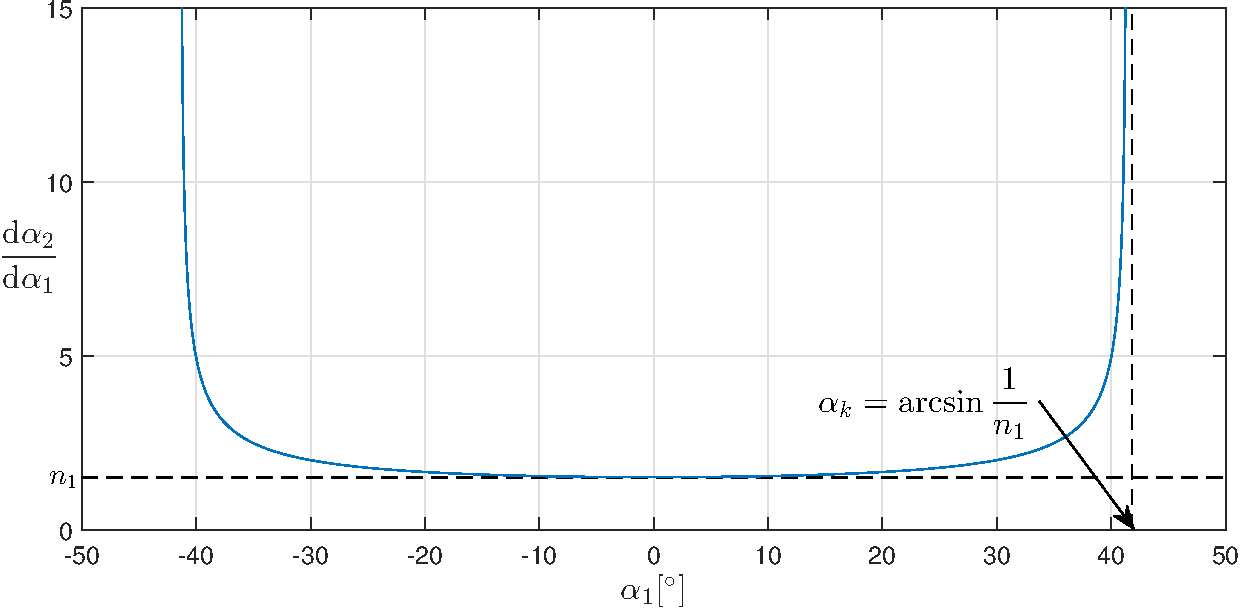
\includegraphics[width = 0.8\linewidth]{derivace.pdf}
\end{center}
\caption[Závislost změny lomeného úhlu na změně úhlu dopadu.]{Závislost změny lomeného úhlu na změně úhlu dopadu. Pro kritický úhel $\alpha_k$ roste k~nekonečnu. Graf funkce popsané vzorcem \ref{eq:zmena velikosti posunu}.}
\label{fig:derivace uhlu}
\end{figure}



\section{Modelování pohybu svazků}
V programu LADOK jsme provedli experiment s rotací broušeného kamene \textit{viva12}.

Rotací kamene okolo osy kolmé ke spodku kamene dostaneme pouze soustředné kružnice. Kámen jsme tedy rotovali kolem vodorovné osy procházející středem spodku kamene o konstantní úhel v každém kroku. Zaznamenali jsme směry vystupujících svazků při různých pozicích kamene. Výsledek jsme vykreslili do polárního grafu. Ze dvou po sobě následujících pozic kamene jsme šipkou spojili pozici svazků se stejným seznamem dopadových faset. Výsledný obrazec je znázorněn na obr. \ref{fig:relativni pohyb graf}.

Z praktického hlediska nás mohou zajímat pouze svazky, které vytvoří po dopadu na stínítko detekovatelnou stoupu.

% obrazek pohybu jednotlivych stop 
\begin{figure}[h!]
\begin{center}
   \begin{minipage}[c]{0.48\textwidth}
     \centering 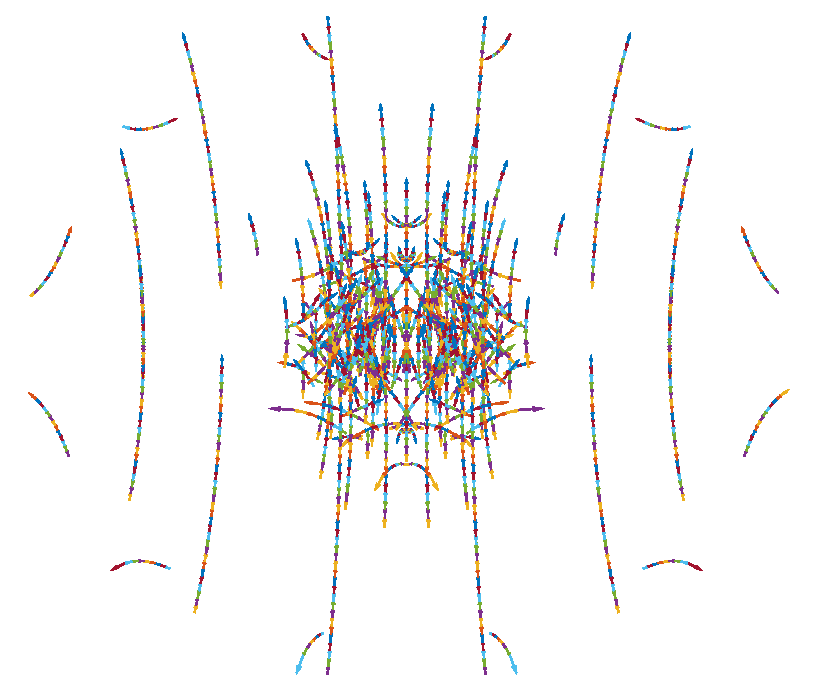
\includegraphics[width = 1\linewidth]{viva12_bigflux.eps}
   \end{minipage}
   \begin{minipage}[c]{0.48\textwidth}
     \centering 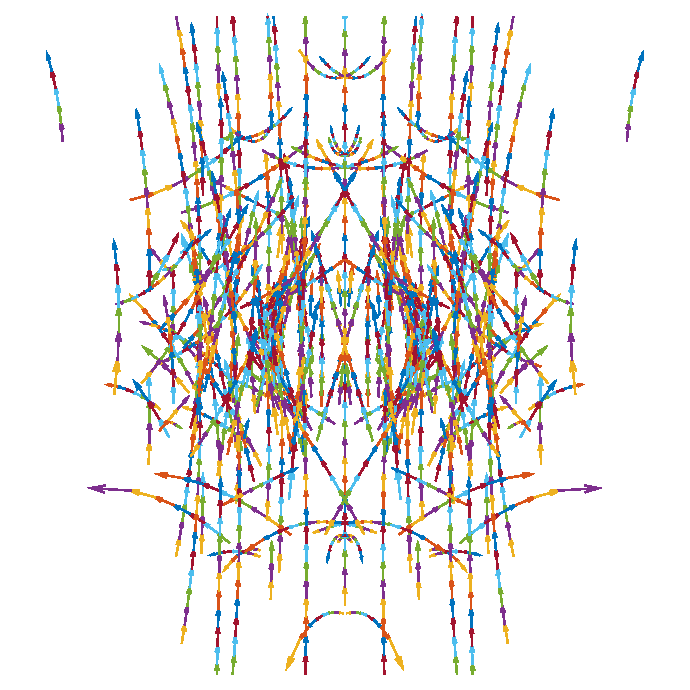
\includegraphics[width = 1\linewidth]{viva12_bigflux2.eps}
   \end{minipage}
 \end{center}
\caption[Dráhy pohybu svazků při rotaci kamene.]{Dráhy směru svazků vycházejících z kamene \textit{viva12} získané pomocí simulačního programu  LADOK při rotaci kamene. Zobrazeny jsou pouze svazky s významným zářivým tokem vycházející v horního poloprostoru kamene. Vpravo detail na střed obrázku vlevo.}

\label{fig:relativni pohyb graf}
\end{figure}

Pro lepší představu o změně směru jednotlivých svazků nám může být užitečný kruhový histogram znázorňující směr jejich pohybu (obr. \ref{fig:relativni pohyb graf}). Podstatná většina svazků se posouvá ve směru rotace kamene, což není příliš nápomocné při jejich identifikaci.

Existují však svazky, které jsou svým pohybem charakteristické a lze je tedy oddělit od ostatních. Kritérium pro rozpoznání svazků nemusí být pouze směr pohybu, ale jak vidíme na obr. \ref{fig:relativni pohyb graf} i velikost úhlu rotace. V neposlední řadě přichází v úvahu i změna zářivého toku svazků, změna velikosti ocásků a další. 

\begin{figure}[h!]
 \begin{center}
   \begin{minipage}[c]{0.48\textwidth}
     \centering 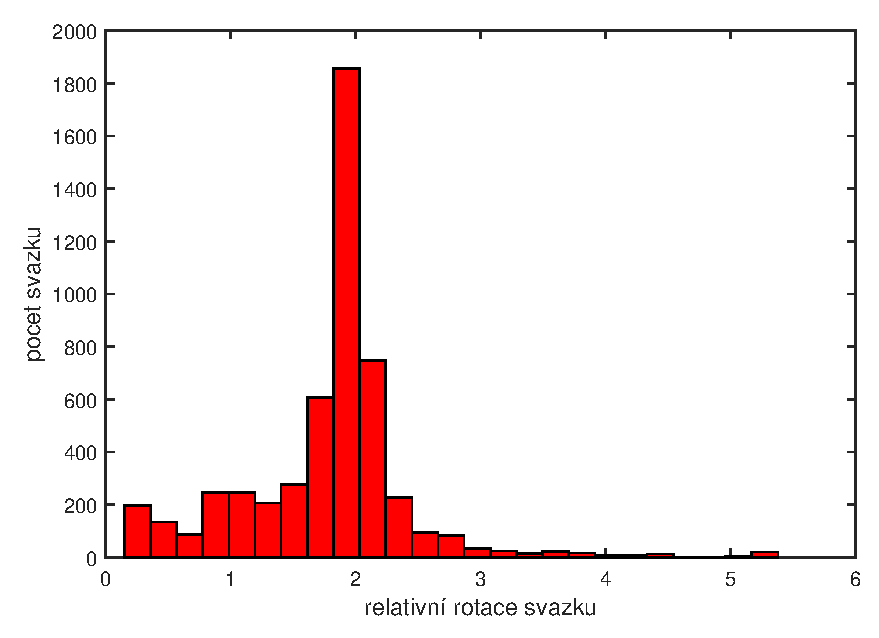
\includegraphics[width = \linewidth]{relative.eps} 
   \end{minipage}
   \begin{minipage}[c]{0.48\textwidth}
     \centering 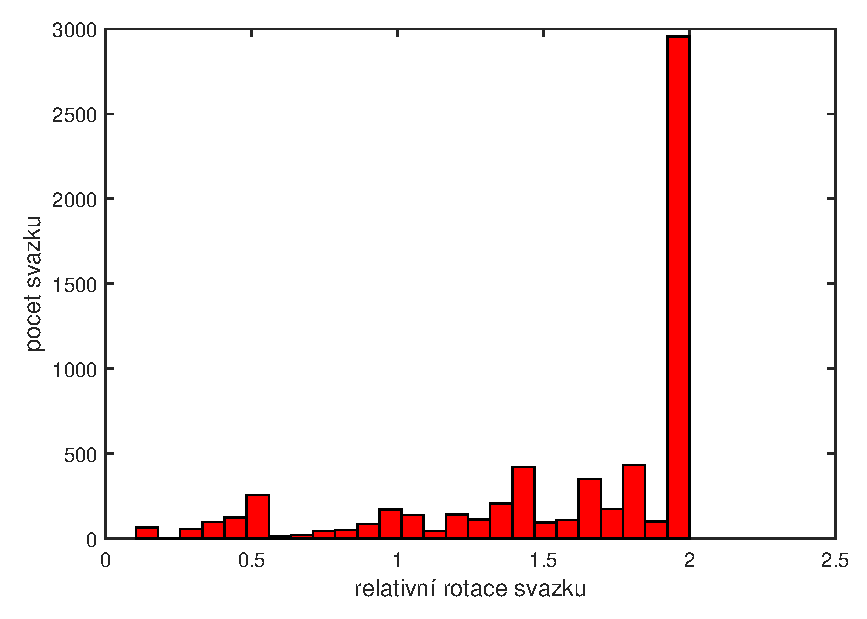
\includegraphics[width =\linewidth]{relative_index1.eps} 
   \end{minipage}
 \end{center}
\caption[Histogram velikosti rotace vystupujících svazků.]{Vlevo: histogram velikosti úhlu rotace vystupujících svazků z kamene \textit{viva12} z obrázku \ref{fig:relativni pohyb graf}. Vlivem lomu je relativní rotace v mnoha případech větší než 2. V okolí kritického úhlu roste k~nekonečnu. Pokud ztotožníme indexy lomu kamene a okolí, tak relativní rotace nebude větší než 2. To lze vidět na histogramu vpravo.}

\label{fig:histogram relativni pohyb }

\end{figure}

Vykresleme si histogram (obr. \ref{fig:histogram relativni pohyb } vlevo) relativní velikosti úhlu rotace vystupujících svazků. Z něj je patrné, že řada svazků rotuje o více než dvojnásobek úhlu rotace kamene $\alpha$, což potvrzuje teorii o relativní změně směru svazků z rovnice \ref{eq:zmena velikosti posunu}. 



\begin{figure}[h!]
\begin{center}
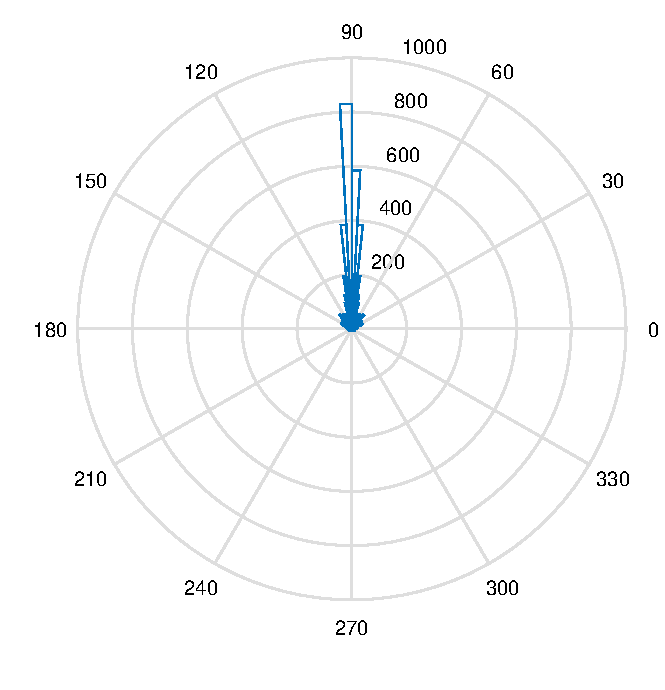
\includegraphics[width =0.7\linewidth]{kruhovy_histogram.eps}
\end{center}
\caption[Kruhový histogram směru rotace svazků - \textit{viva12}.]{Kruhový histogram směru rotace vystupujících svazků kamene \textit{viva12} z obrázku \ref{fig:relativni pohyb graf}. Většina svazků se pohybuje ve směru rotace kamene.}
\label{fig:kruhovy histogram}
\end{figure}

Pokud vezmeme kámen o stejném indexu lomu, jako je okolí, nedochází k lomu. Potom by se nemělo docházet k rotaci výstupního svazku o úhel větší než $2\alpha$, způsobená právě rozdílným indexem lomu. Pro potvrzení této teorie jsme provedli stejnou simulaci jako v~předchozím případě. Indexy lomu kamene a jeho okolí jsme ztotožnili a výsledek simulace ukázal, že rotace výstupních svazků úhel větší než $2\alpha$ se již nevyskytují. To nám dokládá zhotovený histogram (obr. \ref{fig:histogram relativni pohyb } vpravo).


Téměř konstantní směrovost rotace svazků u kamene \textit{viva12} zmenšuje význam příspěvku této vlastnosti k lepšímu rozpoznání světelných stop. Pokud ovšem provedeme stejný experiment na broušeném kameni jiného tvaru, dostaneme rozdílný výsledek. Například u šatonu, svým tvarem složitějším než \textit{viva12}, je směr rotace svazků rozmanitější. Velká část z nich samozřejmě rotuje ve směru rotace kamene. Jak ale vidíme z kruhového histogramu (obr. \ref{fig:kruhovy histogram saton}), lze rozlišovat i velké množství stop pohybujících se např. pod úhlem $45^\circ$. U šatonu tedy může znalost směru pohybu svazků při rotaci kamene nemalou měrou pomoci v jejich rozpoznání. 

\begin{figure}
\begin{center}
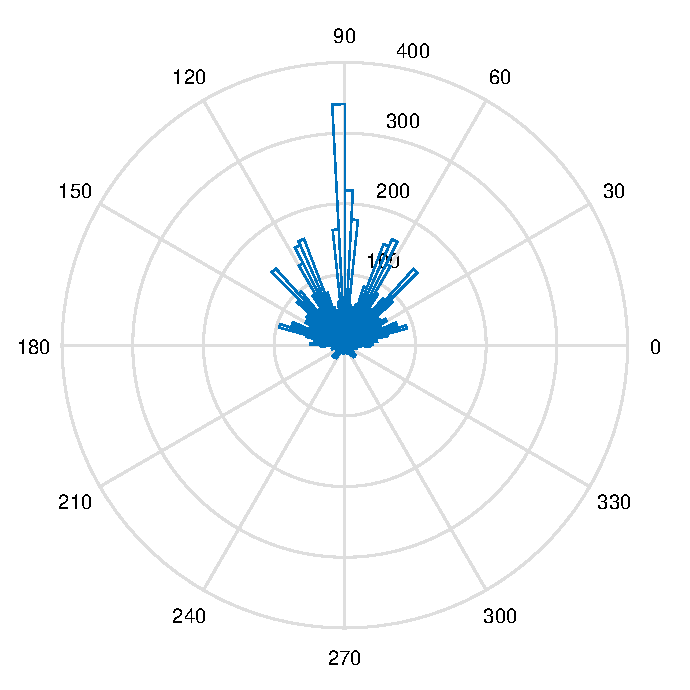
\includegraphics[width = 0.7\textwidth]{saton_smer.eps}
\end{center}
\caption[Kruhový histogram směru rotace svazků - šaton.]{Kruhový histogram směru rotace vystupujících svazků z šatonu při rotaci kamene.}

\label{fig:kruhovy histogram saton}
\end{figure}

  
\clearpage

%\begin{figure}[htbp]
%    \resizebox{\linewidth}{!}{ \input{figures/tailex07.pdf_tex}} % specify figure name
%\end{figure}
	
%\bibliographystyle{unsrt}	
\clearpage
\nocite{*}
\printbibliography 

\end{document}
